\documentclass[11pt]{amsart}

\usepackage[margin=1in]{geometry}
\usepackage{mathptmx}
\usepackage{amssymb}
\usepackage{graphicx}
\usepackage{booktabs}
\usepackage{xcolor}
\usepackage{enumitem}
\usepackage{xurl}
\usepackage[colorlinks=true,linkcolor=blue!50!black,citecolor=blue!50!black,urlcolor=blue!50!black,bookmarksnumbered=true]{hyperref}
\usepackage{microtype}

\tolerance=2000
\emergencystretch=3em
\raggedbottom

\newtheorem{theorem}{Theorem}
\newtheorem{lemma}[theorem]{Lemma}
\newtheorem{proposition}[theorem]{Proposition}
\newtheorem{corollary}[theorem]{Corollary}
\theoremstyle{definition}
\newtheorem{definition}[theorem]{Definition}
\newtheorem{conjecture}[theorem]{Conjecture}
\theoremstyle{remark}
\newtheorem{remark}[theorem]{Remark}

\newcommand{\R}{\mathbb{R}}
\newcommand{\Z}{\mathbb{Z}}
\newcommand{\C}{\mathbb{C}}
\newcommand{\Q}{\mathbb{Q}}
\newcommand{\PP}{\mathbb{P}}
\newcommand{\cL}{\mathcal{L}}
\newcommand{\cM}{\mathcal{M}}
\newcommand{\cS}{\mathcal{S}}
\newcommand{\cV}{\mathcal{V}}
\newcommand{\cO}{\mathcal{O}}
\newcommand{\Hom}{\operatorname{Hom}}
\newcommand{\End}{\operatorname{End}}
\newcommand{\Hess}{\operatorname{Hess}}
\newcommand{\Res}{\operatorname{Res}}
\newcommand{\rk}{\operatorname{rank}}
\newcommand{\ip}[2]{\langle #1,#2\rangle}
\newcommand{\bb}{\mathbf{b}}
\newcommand{\cc}{\mathbf{c}}
\newcommand{\va}{\mathbf{a}}
\newcommand{\ee}{\mathbf{e}}
\newcommand{\one}{\mathbf{1}}
\newcommand{\WP}{\mathrm{WP}}

\setlength{\emergencystretch}{3em}

\begin{document}

\title{Which String Vibrations Become Which Generations on the Dwork Quintic}

\author{Deep Bhattacharjee}
\address{Formerly, Electro-Gravitational Space Propulsion Laboratory (EGSPL), Bhubaneswar, Odisha 751030, India}
\address{Formerly, University of Calcutta, Senate House, 87/1 College Street, Kolkata 700073, West Bengal, India}
\email{itsdeep@live.com}
\urladdr{\href{https://orcid.org/0000-0003-0466-750X}{https://orcid.org/0000-0003-0466-750X}}
\thanks{Corresponding author; second e-mail address \nolinkurl{d.bhattacharjee@erl-forschung.de}}

\author{Ushashi Bhattacharya}
\address{Formerly, National Taiwan University, Taipei 106319, Taiwan}
\email{rai.bhattacharya.in@gmail.com}
\urladdr{\href{https://orcid.org/0009-0002-2254-3914}{https://orcid.org/0009-0002-2254-3914}}

\subjclass[2020]{Primary 14J32, 81T30; Secondary 14D07, 32G20, 14J33, 20C15, 13H10, 81R05}
\keywords{heterotic string, quintic threefold, Yukawa couplings, generations, free quotients}

\begin{abstract}
We determine, for the heterotic string on the one-parameter family of
quintic threefolds, which vibration modes become which families of charged
particles. The hundred and one families are labelled by the characters of a
symmetry group of order one hundred and twenty-five. Every Yukawa coupling
that this symmetry allows is a power of the modulus, and every other
coupling vanishes. The invariant deformation pairs each family with exactly
one partner, so that fifty families are massless at the Fermat point and
none anywhere else, and at the Fermat point the masses are given in closed
form by the Gamma function. On the three other one-parameter families of
the same type, in weighted projective spaces, the symmetry no longer tells
the families apart and some families stay massless at every member. We
also prove that the Geometric Selection Conjecture is equivalent to the
existence of one viable vacuum fixed by mirror symmetry, and that a free
quotient of a Calabi--Yau complete intersection of any of the thirteen
one-parameter hypergeometric types never carries three families with the
standard embedding; on seven of these types, among them the sextic and
dectic pencils, no finite group acts freely at all.
\end{abstract}

\maketitle


\setcounter{tocdepth}{1}
\tableofcontents

\section{Introduction}\label{sec:intro}

A closed string moving in ten dimensions has a tower of vibration modes, and
the massless ones of the heterotic string on a product of four-dimensional
space-time with a compact six-manifold $X$ are the fields of a
four-dimensional gauge theory. When $X$ is a Calabi--Yau threefold and the
gauge connection is identified with the Levi-Civita connection of its
Ricci-flat metric, the gauge group is $E_6$ and the charged chiral multiplets
come in two conjugate representations whose numbers are the two Hodge numbers
of $X$. This was established in 1985 by Candelas, Horowitz, Strominger and
Witten~\cite{CHSW85} and by Witten~\cite{Wit85}, and the couplings of three
charged fields were identified by Strominger~\cite{Str85} with an integral
over $X$ that Candelas~\cite{Can88} computed on the quintic threefold.
The question in the title is the one that this dictionary leaves open: a
vibration mode is a cohomology class on $X$, a particle generation is an
irreducible piece of the four-dimensional spectrum, and one wants to know
which class carries which generation, with what mass, and how this changes as
$X$ moves in its moduli space.\footnote{The word generation is used here in
the sense of the $E_6$ theory: one copy of the representation $\mathbf{27}$,
which contains one family of quarks and leptons together with its Higgs
and singlet partners. The three observed families are three such copies
after the further breaking of $E_6$; the paper does not touch that
breaking, which depends on discrete Wilson lines and on a quotient of $X$
that the quintic does not admit in a form that reduces a hundred and one
copies to three, so that the results here concern the full $E_6$ spectrum
of the covering space.}

We answer it completely on one family, the Dwork pencil of quintics
\begin{equation}\label{eq:dwork}
X_\psi=\{x_1^5+x_2^5+x_3^5+x_4^5+x_5^5-5\psi\,x_1x_2x_3x_4x_5=0\}\subset\PP^4,
\end{equation}
smooth for $\psi^5\ne1$, which is the family on which mirror symmetry was
first tested by Candelas, de la Ossa, Green and Parkes~\cite{CDGP91} and on
which the Yukawa couplings were counted by Doran, Greene and
Judes~\cite{DGJ08}. The group $\Gamma\cong(\Z/5)^3$ of diagonal phases
preserving the equation acts on every member of the pencil, and the
hundred and one classes in $H^{2,1}(X_\psi)$, which are the hundred and one
copies of the $\mathbf{27}$, are the monomials $x^{\bb}$ with exponent
vector $\bb\in\{0,1,2,3\}^5$ of total degree five. The results are the
following.

\begin{theorem}[Labels]\label{thm:A}
The hundred and one classes carry hundred and one distinct characters of
$\Gamma$, each with multiplicity one, so every generation is labelled by
its character. Of the hundred and twenty-five characters of $\Gamma$ the
twenty-four that do not occur are exactly the classes of the permutations
of $(0,1,2,3,4)$. The permutation group $S_5$ of the coordinates permutes
the labels in five orbits of sizes $1$, $20$, $20$, $30$ and $30$, the five
types of generation.
\end{theorem}

\begin{theorem}[Couplings]\label{thm:B}
Let $\psi^5\ne1$. The cubic form of the pencil, normalised so that the
monomial $x_1^3\cdots x_5^3$ has value one, takes on three generations
$\va,\bb,\cc$ the value $\psi^{r}$ when $\va+\bb+\cc\equiv(3-r)\one\pmod 5$
for some $r\in\{0,1,2,3\}$, and zero otherwise. There are $1431$ unordered
triples with a nonzero coupling, $566$, $425$, $280$ and $160$ of them with
$r=0,1,2,3$, and all $1431$ are nonzero at every smooth member with
$\psi\ne0$.
\end{theorem}

\begin{theorem}[Mass map]\label{thm:C}
The invariant class $h=x_1x_2x_3x_4x_5$, the direction of the pencil
itself, pairs each generation $\bb$ with exactly one generation
$\sigma(\bb)$, where $\sigma$ is an involution of the labels with one fixed
point. The coupling of $h$, $\bb$ and $\sigma(\bb)$ equals $1$ for the
fifty-one labels with all entries at most two, $\psi$ for the thirty labels
of type $(3,1,1,0,0)$ and $\psi^2$ for the twenty labels of type
$(3,2,0,0,0)$. Hence the mass matrix induced by a vacuum value of the
$\mathbf{27}$ labelled by $h$ has full rank one hundred and one for every
$\psi\ne0$, $\psi^5\ne1$, its determinant is $\psi^{70}$, and at the
Fermat point $\psi=0$ its rank is fifty-one with the fifty generations
containing an exponent three massless. The spectrum consists of one singlet
and fifty doublets, and the $\Gamma$-invariant metric is diagonal in the
labels, so the fifty doublet masses are, in units of the vacuum value,
$|\psi|^{r(\bb)}\big(g_{\bb}\,g_{\sigma(\bb)}\big)^{-1/2}$ with $g$ the
Hodge norms of the classes.
\end{theorem}

Theorem~\ref{thm:B} is stronger than the count of Doran, Greene and
Judes~\cite{DGJ08}, who found by a search that $1431$ couplings are allowed
by the symmetry; it shows that the symmetry is the only source of zeros, and
gives every allowed coupling in closed form. The number $1431$ is recovered
by hand in Section~\ref{sec:count}. The theorems are proved in
Sections~\ref{sec:labels} to~\ref{sec:mass} after the dictionary between
vibrations and particles is set out, with complete proofs, in
Section~\ref{sec:dictionary}. Section~\ref{sec:fermat} evaluates the Hodge
norms at the Fermat point in terms of the Gamma function, which turns the
mass formula of Theorem~\ref{thm:C} into numbers there.

The fourth result concerns the choice of the vacuum. A conjecture of
Bhattacharjee, Bhattacharya and Ghosh~\cite{Bha26a}, the Geometric Selection
Conjecture, asks for a functional on the heterotic landscape, built from the
Weil--Petersson metric, that is proper, has a unique minimum, takes that
minimum at a phenomenologically viable vacuum and is invariant under mirror
symmetry. The precise statement is recalled in Section~\ref{sec:selection}.

\begin{theorem}[Selection]\label{thm:D}
The Geometric Selection Conjecture holds if and only if there is a viable
vacuum, in the sense of conditions \textup{(C1)} to \textup{(C9)}
of~\cite{Bha26a}, that is not moved by the mirror involution. On the Dwork
pencil the mass condition \textup{(C8)} holds in the precise form that the
mass map of the invariant direction has full rank with entries $1$,
$\psi$ and $\psi^2$, at every member with $\psi\ne0$; the three-family
condition \textup{(C2)} fails on every smooth quintic and on every quotient
of a smooth quintic by a group acting freely.
\end{theorem}

The first part says that the functional carries no information beyond the
vacuum it selects: once a viable vacuum is given, a functional with all the
required properties is written down in Section~\ref{sec:selection} from the
metric alone, and conversely the minimum of any such functional is a viable
vacuum. What remains of the conjecture is therefore the existence of one
viable vacuum, which is where its content lies. The second part locates the
Dwork pencil with respect to that question: its mass spectrum has the full
rank and the hierarchy of scales that condition (C8) asks for, and the
obstruction is the number of families, a hundred and one on the quintic and
$100/|H|$ on a free quotient by a group $H$, never three.

The same questions can be asked of the three other one-parameter families
of Fermat type, the pencils
\begin{equation}\label{eq:wpencil}
X_\psi=\Big\{\sum_{i=1}^5x_i^{n_i}-d\psi\,x_1x_2x_3x_4x_5=0\Big\}
\subset\PP(w),\qquad n_i=\frac{d}{w_i},
\end{equation}
of sextics in $\PP(1,1,1,1,2)$, octics in $\PP(1,1,1,1,4)$ and dectics in
$\PP(1,1,1,2,5)$, whose periods and mirror maps were computed by
Morrison~\cite{Mor92}, Klemm and Theisen~\cite{KT93} and
Font~\cite{Fon93}. Here $d=\sum_iw_i$ is $6$, $8$ and $10$, each member
with $\psi^d\delta\ne1$, where $\delta=\prod_iw_i^{w_i}$ is $4$, $256$ and
$12\,500$, is smooth, and the group $\Gamma$ of diagonal phases preserving
the pencil has order $108$, $128$ and $100$. The answer is different there.

\begin{theorem}[Weighted pencils]\label{thm:E}
Let $X_\psi$ be the sextic, octic or dectic pencil \eqref{eq:wpencil} with
$\psi^d\delta\ne1$. Then $X_\psi$ is a smooth Calabi--Yau threefold with
$h^{1,1}=1$ and $h^{2,1}=103$, $149$ and $145$, and the following hold.
\begin{enumerate}[label=\textup{(\roman*)},leftmargin=*,itemsep=1pt]
\item The generations are the monomials $x^{\bb}$ of weighted degree $d$
with $0\le b_i\le n_i-2$, but they carry only $96$, $122$ and $100$
distinct characters of $\Gamma$: $7$, $27$ and $42$ classes of two or three
generations share a character.
\item The cubic form, normalised so that $\prod_ix_i^{n_i-2}$ has value
one, takes on three generations $\va,\bb,\cc$ the value
$\psi^r\prod_iw_i^{k_i}$ when $a_i+b_i+c_i=n_i-2-r+n_ik_i$ for every $i$,
with $r\in\{0,\dots,d-1\}$ and integers $k_i\ge0$, and zero otherwise; for
$\psi\ne0$ every coupling allowed by $\Gamma$ is nonzero.
\item For $\psi\ne0$ the mass map of the invariant direction has rank
$99$, $125$ and $109$, so that $4$, $24$ and $36$ generations stay massless
at every member; at $\psi=0$ its rank is $44$, $85$ and $72$.
\item No member, and no quotient of a member by a group acting freely,
carries three families with the standard embedding.
\end{enumerate}
\end{theorem}

So the two properties that make the Dwork pencil transparent are special
to it. On the weighted pencils a shift of the exponents at the coordinates
of weight one can be balanced by a shift at the coordinate of larger
weight, the characters of $\Gamma$ no longer label the generations, and the
massless generations all lie in the span of the classes that share a
character. The precise form of the mass condition (C8) in
Theorem~\ref{thm:D} therefore fails on all three pencils, and so does the
three-family condition (C2). Theorem~\ref{thm:E} is proved in
Section~\ref{sec:weighted}, and Figure~\ref{fig:weighted} compares the four
pencils.

The count of families reaches beyond the four pencils. Of the fourteen
one-parameter families of Calabi--Yau threefolds with hypergeometric
Picard--Fuchs equations, thirteen are complete intersections in weighted
projective space, and Proposition~\ref{prop:freequot} shows that a finite
group acting freely on a smooth member has order divisible only by the
primes that divide the greatest common divisor $g_X$ of the holomorphic
Euler characteristics $\chi(X,\cO_X(k))$, $k\ge1$. This number is $1$ for
seven of the thirteen types, the sextic and the dectic among them, which
therefore have no free quotient at all, and no free quotient of any of the
thirteen carries three families.

The constructions behind the four theorems were organised on the Anaxia
engine of the BLLM programme~\cite{Ana26,BB26}.\footnote{Anaxia runs a
failure-driven loop: each strategy for a target is a list of checks, each
check is a computation or a proof with a named source, a failed check is
recorded together with the change of strategy it forces, and the label of a
target (open, candidate, proved) is computed by the engine from the record,
never assigned by hand. For this paper the engine ran five targets. For the
couplings, the first strategy was the count of couplings allowed by the
symmetry, as in~\cite{DGJ08}; its check that the allowed couplings are
nonzero failed, because a symmetry count only bounds the number of nonzero
couplings from above, and the change it forced was to evaluate the socle
functional of Section~\ref{sec:socle} on every monomial of degree fifteen,
which passed. For the mass map the single strategy, the pairing by the
invariant class, passed at once. For the Fermat point the engine checked the
Gamma-function norms against the constant of Distler and
Greene~\cite{DG88}. For the selection conjecture the first strategy was to
look for the viable vacuum on the quintic itself; its check of the number
of families failed for the quintic and for each of its free quotients, and
the change it forced was to separate the functional from the vacuum, which
gives Theorem~\ref{thm:D}; the check of the existence of a viable vacuum
then failed on the literature, and that target stays open. For the
weighted pencils the first strategy was to carry the proof of
Theorem~\ref{thm:A} over; its check that the characters are distinct
failed at once on the sextic, where $103$ generations carry $96$
characters, and the change it forced was to classify the generations that
share a character by the wrapping of Lemma~\ref{lem:wwrap} and to compute
the mass map block by block, which gives Theorem~\ref{thm:E}. The record
of all five targets was made on release 3.1.0 of the engine. The engine
proposes no mathematics of its own here: every statement is proved in the
text, and the record of the loop is part of the archive of the
paper~\cite{Repo}.}


\subsection*{History}

The dictionary between the vibrations of the string and the fields in four
dimensions on a Calabi--Yau background was written down in~\cite{CHSW85};
the
decomposition of the adjoint of $E_8$ under $E_6\times SU(3)$ and the
identification of the massless charged fields with the Dolbeault cohomology
of the tangent bundle are there, and the identification of the number of
generations with half the Euler characteristic. Witten~\cite{Wit85}
discussed the breaking of $E_6$ by Wilson lines and the pattern of masses
from vacuum values of the $\mathbf{27}$, which is the mechanism behind
Theorem~\ref{thm:C}. Strominger~\cite{Str85} identified the cubic couplings
of the $\mathbf{27}$ with the cubic form on $H^1(X,T_X)$ given by the
holomorphic three-form, and the normalisation by the K\"ahler metric of the
matter fields was clarified by Dixon, Kaplunovsky and Louis~\cite{DKL90}
and by Candelas and de la Ossa~\cite{CdlO91}. Candelas~\cite{Can88}
computed the couplings on the Fermat quintic through the Jacobian ring, with
the Gamma-function normalisation of the Hodge norms at that point; Greene
and Plesser~\cite{GP90} introduced the quotient of the Dwork pencil by
$\Gamma$ as the mirror of the quintic, and~\cite{CDGP91} computed the
coupling of $h$ with itself along the pencil, $5/(1-\psi^5)$ in their
normalisation, which is the case $\va=\bb=\cc=h$ of Theorem~\ref{thm:B}
together with Remark~\ref{rem:hessian}. Doran, Greene and
Judes~\cite{DGJ08} counted by computer the couplings not forced to vanish
by $\Gamma$, found $1431$, and observed that the count is close to the
total divided by the order of the group. The Jacobian-ring description of $H^{2,1}$ of a hypersurface and
of its cubic form is Griffiths'~\cite{Gri69}, and the perfectness of the
residue pairing with the Hessian in the socle is Macaulay's theorem in the
form given by Carlson and Griffiths~\cite{CG80}. On the physical side, the
holomorphic Yukawa couplings of heterotic line-bundle models were computed
by Blesneag, Buchbinder, Candelas and Lukas~\cite{BBCL16}, and the physical,
metric-normalised couplings of the quintic at the Fermat point by Butbaia,
Mayorga Pe\~na, Tan, Berglund, H\"ubsch, Jejjala and Mishra~\cite{BMT24} with
numerical Ricci-flat metrics, whose Gamma-function value for the invariant
direction agrees with Section~\ref{sec:fermat}. Heterotic standard models
with three families on other threefolds were constructed by Braun, He, Ovrut
and Pantev~\cite{BHOP05}, Bouchard and Donagi~\cite{BD06} and Anderson,
Gray, Lukas and Palti~\cite{AGLP11,AGLP12}; the question of which classes
carry which families is posed there in a form that depends on the choice of
bundle, and the present paper answers it in the one case where every piece
of the data is explicit. Distler and Greene~\cite{DG88} computed the
normalised couplings of the Gepner model at the Fermat point exactly, and
Section~\ref{sec:fermat} recovers their constant from the Hodge norms. The
monodromy and intersection numbers used there go back to
Pham~\cite{Pha65}, Sebastiani and Thom~\cite{ST71} and
Sakamoto~\cite{Sak74}. Two further aspects of the same compactifications,
the suppression of the electroweak scale by singularities of the threefold
and fibrations of Calabi--Yau manifolds by circles, are treated
in~\cite{Bha26b,Bha25}. The weighted pencils of Section~\ref{sec:weighted}
are the one-parameter models whose Picard--Fuchs equations, periods and
mirror maps were found by Morrison~\cite{Mor92}, Klemm and
Theisen~\cite{KT93} and Font~\cite{Fon93}, and the Hodge theory of
quasi-smooth hypersurfaces in weighted projective space used there is due
to Steenbrink~\cite{Ste77} and Dolgachev~\cite{Dol82}.

\section{The dictionary}\label{sec:dictionary}

Throughout, $X$ is a compact K\"ahler threefold with holonomy exactly
$SU(3)$, so that $X$ has a Ricci-flat K\"ahler metric $g$ by Yau's
theorem, a nowhere vanishing holomorphic three-form $\Omega$, and
$h^{1,0}=h^{2,0}=0$. The tangent bundle $T_X$ with the Levi-Civita
connection is a holomorphic $SU(3)$-bundle with a Hermitian Yang--Mills
connection; this is the standard embedding.

\subsection{Spinors and the Dolbeault complex}

On a K\"ahler manifold of complex dimension $n$ with trivial canonical
bundle the spinor bundle is $S=\bigoplus_{q}\Lambda^{0,q}T^*_X$, and the
Dirac operator of the Levi-Civita connection is $D=\sqrt2(\bar\partial+
\bar\partial^*)$, with the chirality grading given by the parity of $q$
(Hitchin~\cite{Hit74}). If $V$ is a holomorphic Hermitian bundle with a
connection whose curvature is of type $(1,1)$, the Dirac operator twisted by
$V$ is $\sqrt2(\bar\partial_V+\bar\partial_V^*)$ on $\Lambda^{0,\bullet}
\otimes V$, and its kernel is the harmonic representative of
$\bigoplus_q H^{0,q}(X,V)$. This is the only input from spin geometry.

\subsection{The charged spectrum}

\begin{theorem}[Spectrum of the standard embedding]\label{thm:dictionary}
Let $X$ be as above with the standard embedding. The massless charged
chiral multiplets of the $E_8\times E_8$ heterotic string on $\R^{3,1}
\times X$ in the observable sector transform under $E_6$ as
\[
h^{2,1}(X)\ \text{copies of }\mathbf{27}\ \oplus\ h^{1,1}(X)\ \text{copies of
}\overline{\mathbf{27}},
\]
with the $\mathbf{27}$'s in natural bijection with $H^1(X,T_X)\cong
H^{2,1}(X)$ and the $\overline{\mathbf{27}}$'s with $H^1(X,T_X^*)\cong
H^{1,1}(X)$. The net number of generations is
$|h^{2,1}-h^{1,1}|=\tfrac12|\chi(X)|$.
\end{theorem}

\begin{proof}
The ten-dimensional gaugino is a Majorana--Weyl spinor with values in the
adjoint of $E_8$. Under $E_8\supset E_6\times SU(3)$,
\[
\mathbf{248}=(\mathbf{78},\mathbf1)\oplus(\mathbf1,\mathbf8)\oplus
(\mathbf{27},\mathbf3)\oplus(\overline{\mathbf{27}},\bar{\mathbf3}),
\]
and the standard embedding identifies the $SU(3)$ factor with the holonomy
group acting on $T_X$ and sends $\mathbf3$ to $T_X$, $\bar{\mathbf3}$ to
$T_X^*$. A ten-dimensional Weyl spinor on $\R^{3,1}\times X$ decomposes as
a four-dimensional Weyl spinor times a six-dimensional one of correlated
chirality, so the four-dimensional massless chiral fermions in the
$\mathbf{27}$ are the zero modes of the Dirac operator on $X$ twisted by
$T_X$, counted with their six-dimensional chirality; the $SU(3)$ holonomy
makes the twisted operator $\sqrt2(\bar\partial+\bar\partial^*)$ on
$\Lambda^{0,\bullet}\otimes T_X$, and its chiral zero modes are
$H^{0,1}(X,T_X)\oplus H^{0,3}(X,T_X)$ and $H^{0,0}(X,T_X)\oplus
H^{0,2}(X,T_X)$ for the two chiralities. Since $\Omega$ trivialises
$\Lambda^3T_X^*$, contraction with $\Omega$ gives $H^{0,q}(X,T_X)\cong
H^{2,q}(X)$ and $H^{0,q}(X,T_X^*)=H^{1,q}(X)$. With $h^{2,0}=h^{1,0}=0$
and Serre duality, $H^{0,0}(T_X)=H^{2,0}=0$, $H^{0,3}(T_X)=
H^{2,3}=\overline{H^{1,0}}^*=0$, $H^{0,2}(T_X)=H^{2,2}\cong
\overline{H^{1,1}}$, and $H^{0,1}(T_X)=H^{2,1}$. A four-dimensional Weyl
fermion in the $\mathbf{27}$ of one chirality and one in the
$\overline{\mathbf{27}}$ of the opposite chirality are related by
conjugation, so the chiral multiplets of definite four-dimensional
chirality are $h^{2,1}$ copies of $\mathbf{27}$ from $H^{0,1}(T_X)$ and
$h^{1,1}$ copies of $\overline{\mathbf{27}}$ from $H^{0,2}(T_X)$. The index
of the twisted Dirac operator is $h^{2,1}-h^{1,1}$, which equals $-\chi(X)/2$
because $\chi=2(h^{1,1}-h^{2,1})$ on a threefold with $h^{1,0}=h^{2,0}=0$.
\end{proof}

\subsection{The cubic form}

Let $V=H^1(X,T_X)$. The composition of cup product and contraction,
\[
V\otimes V\otimes V\to H^3(X,\Lambda^3T_X)=H^3(X,K_X^{-1})\cong
H^3(X,\cO_X)\cong\C,
\]
where the last two isomorphisms use $\Omega$, is a symmetric trilinear form
$Y$ on $V$, the cubic form of $X$. In terms of the variation of Hodge
structure, with $\nabla$ the Gauss--Manin connection and $\Omega$ extended
holomorphically over the moduli space,
\begin{equation}\label{eq:yukawa}
Y(a,b,c)=\int_X\Omega\wedge\nabla_a\nabla_b\nabla_c\Omega,
\end{equation}
and this is the coupling of three $\mathbf{27}$'s~\cite{Str85}. Changing
$\Omega$ to $f\Omega$ multiplies $Y$ by $f^2$, so only the cubic form up to
a nowhere vanishing holomorphic function is intrinsic, and the physical
couplings are $Y$ divided by the square roots of the Hodge norms of the three
classes and by $\ip{\Omega}{\overline\Omega}$~\cite{DKL90,CdlO91}.

\subsection{Mass terms}

A vacuum value $v$ of the scalar in the $\mathbf{27}$ labelled by a class
$h\in V$ in a direction that breaks $E_6$ gives, through the superpotential
$Y(h,\cdot,\cdot)$, a Dirac mass term $v\,Y(h,b,c)$ between the fermions
labelled by $b$ and $c$~\cite{Wit85}. The physical mass matrix is
\begin{equation}\label{eq:massmatrix}
M_{bc}=v\,\frac{Y(h,b,c)}{\sqrt{g_{b}\,g_{c}}}
\end{equation}
in an orthogonal basis of $V$, where $g_b=\ip{\omega_b}{\overline{\omega_b}}$
is the Hodge norm of the harmonic representative, and the masses are its
singular values. We call $Y(h,\cdot,\cdot)$ the mass map of $h$.

\subsection{Hypersurfaces}

For a smooth hypersurface $X=\{F=0\}\subset\PP^4$ of degree five let
$J_F=(\partial_1F,\dots,\partial_5F)$ be the Jacobian ideal and
$R=\C[x_1,\dots,x_5]/J_F$ the Jacobian ring, graded by degree. Griffiths'
theorem~\cite{Gri69} identifies $H^{3-q,q}_{\mathrm{prim}}(X)$ with
$R_{5(q+1)-5}$ through residues: for a homogeneous $P$ of degree $5q$,
\[
\omega_P=\Res_X\frac{P\,\Omega_0}{F^{q+1}},\qquad
\Omega_0=\sum_i(-1)^{i}x_i\,dx_1\wedge\cdots\widehat{dx_i}\cdots\wedge dx_5,
\]
so $H^{3,0}=R_0$, $H^{2,1}=R_5$, $H^{1,2}=R_{10}$, $H^{0,3}=R_{15}$, and
every class of a quintic threefold is primitive in degree three. The ring
$R$ is a graded complete intersection with Hilbert series
$(1+t+t^2+t^3)^5$, so $\dim R_5=101$, $\dim R_{15}=1$, and $R_{15}$ is the
socle. Macaulay's theorem, as stated in~\cite{CG80}, says that the Hessian
$\Hess F=\det(\partial_i\partial_jF)$ has nonzero image in $R_{15}$ and
that the cubic form is multiplication in $R$ followed by the residue
functional $\lambda_F:R_{15}\to\C$, $\lambda_F(\Hess F)=1$, up to a
constant depending only on the normalisation of $\Omega$:
\begin{equation}\label{eq:jacobianyukawa}
Y(\omega_P,\omega_Q,\omega_S)=c\,\lambda_F(PQS).
\end{equation}
Figure~\ref{fig:hodge} shows a curve on the Fermat quintic and the Hodge
numbers of a quintic threefold: by Theorem~\ref{thm:dictionary} the hundred and one classes
of type $(2,1)$ are the generations and the single class of type $(1,1)$
is the antigeneration.

\begin{figure}[t]
\centering
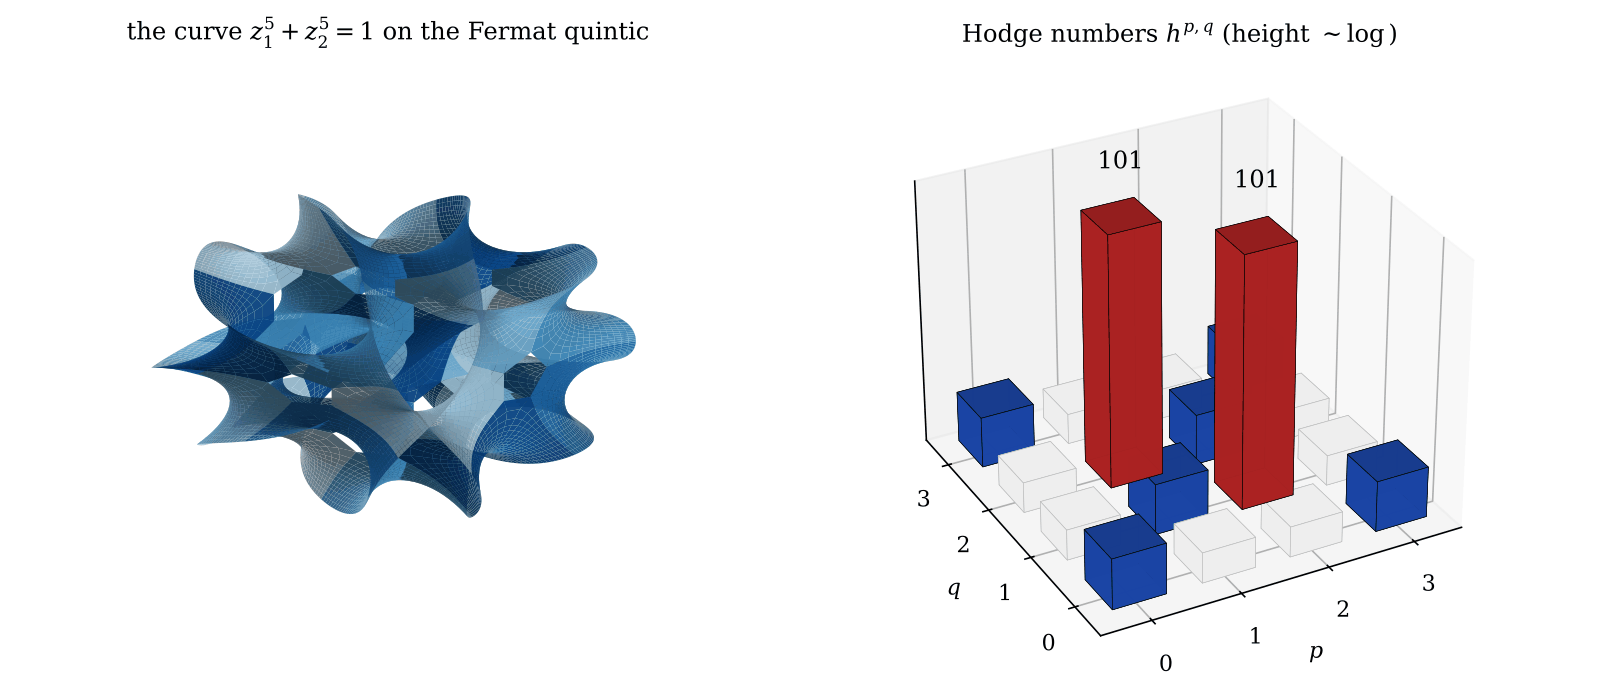
\includegraphics[width=0.96\textwidth]{figures/fig_hodge.png}
\caption{Left: the intersection of the Fermat quintic with the plane
$x_3=x_4=0$, which in an affine chart is the curve $z_1^5+z_2^5=1$ in
$\C^2$, drawn with the parametrisation of Hanson~\cite{Han94} and projected
to three dimensions along $(\mathrm{Re}\,z_1,\mathrm{Re}\,z_2,
\cos\alpha\,\mathrm{Im}\,z_1+\sin\alpha\,\mathrm{Im}\,z_2)$. It is
assembled from twenty-five patches, one for each pair of fifth roots of
unity; $\Gamma$ preserves the curve and acts on it through
$\mu_5\times\mu_5$, permuting the patches. Right:
the Hodge numbers $h^{p,q}$ of a smooth quintic threefold, with height
proportional to $1+\log_2h^{p,q}$; the six blue bars have height one, the
two red bars are $h^{2,1}=h^{1,2}=101$, and the grey cells are zero.}
\label{fig:hodge}
\end{figure}

\section{Labels}\label{sec:labels}

Let $\zeta=e^{2\pi i/5}$ and let $K=\{a\in(\Z/5)^5:\sum a_i=0\}$ act on
$\PP^4$ by $x_i\mapsto\zeta^{a_i}x_i$. The diagonal subgroup $D$ acts
trivially on $\PP^4$, and $\Gamma=K/D\cong(\Z/5)^3$ preserves $F_\psi=
\sum x_i^5-5\psi\prod x_i$ for every $\psi$. The characters of $\Gamma$ are
the characters of $K$ trivial on $D$, that is the classes
\[
\widehat\Gamma=\{\bb\in(\Z/5)^5:\textstyle\sum b_i=0\}/\langle\one\rangle,
\qquad |\widehat\Gamma|=125,
\]
with $\bb$ acting by $a\mapsto\zeta^{a\cdot\bb}$. A monomial $x^{\bb}$
transforms under $a\in K$ by $\zeta^{a\cdot\bb}$, so it lies in the isotypic
component of the class of $\bb$.

Let $B$ be the set of $\bb\in\{0,1,2,3\}^5$ with $|\bb|=\sum b_i=5$. The
monomials $x^{\bb}$, $\bb\in B$, are a basis of $R_5$ for $\psi^5\ne1$,
because the Jacobian ideal of $F_\psi$ is generated by $x_i^4-\psi\prod_{j
\ne i}x_j$, and modulo these every monomial reduces to one with all
exponents at most three; the reduced monomials of degree five are the
$101$ elements of $B$, which matches $\dim R_5$. The count is the number of
compositions of five into five parts, $\binom94=126$, less the twenty with
a part equal to four and the five with a part equal to five.

\begin{proof}[Proof of Theorem~\ref{thm:A}]
Two elements $\bb,\bb'\in B$ define the same character when
$\bb'\equiv\bb+k\one\pmod5$ for some $k$. Since the entries of $\bb'$ lie in
$\{0,\dots,4\}$, $\bb'$ is the vector of residues of $\bb+k\one$ in that
range: each $b'_i$ is $b_i+k$ or $b_i+k-5$, and $\sum b'_i=5$. For $k=1$ the
residues are $b_i+1\le4$ unless $b_i=4$, impossible, so all residues are
$b_i+1$, with sum $10\ne5$. For $k=2$ the residues are $b_i+2$ if $b_i\le2$
and $b_i-3$ if $b_i=3$; the sum is $15-5m$ where $m$ is the number of
threes, so $m=2$, but two threes already sum to six. For $k=3$ the residues
are $b_i+3$ if $b_i\le1$ and $b_i-2$ if $b_i\ge2$, sum $20-5m'$ with $m'$
the number of entries at least two, so $m'=3$, three entries at least two
summing to at most five, impossible. For $k=4$ the residues are $b_i+4$ if
$b_i=0$ and $b_i-1$ otherwise, sum $25-5m''$ with $m''$ the number of
nonzero entries, so $m''=4$: four nonzero entries summing to five means
$(2,1,1,1,0)$ up to order, and then $\bb'=(1,0,0,0,4)$ has a four. So only
$k=0$ works and the $101$ characters are distinct; being characters of an
abelian group acting on $R_5$, they are then the full decomposition, each
isotypic component being one-dimensional.

The group $\widehat\Gamma$ has $125$ elements and $B$ realises $101$ of
them, so exactly $24$ are missed. A permutation of $(0,1,2,3,4)$ has sum
ten, so its class lies in $\widehat\Gamma$, and adding $\one$ to it gives
another permutation of $(0,1,2,3,4)$ modulo five; the hundred and twenty
permutations therefore fall into $24$ classes of five. None of these classes
meets $B$, because every representative with entries in $\{0,\dots,4\}$
is a permutation of $(0,1,2,3,4)$ and contains a four. Hence the $24$ missed
classes are exactly the classes of the permutations.

Finally $S_5$ permutes the exponent vectors, and the orbits in $B$ are the
multisets of entries: $\{1,1,1,1,1\}$ (one element), $\{2,1,1,1,0\}$
(twenty), $\{3,2,0,0,0\}$ (twenty), $\{2,2,1,0,0\}$ (thirty) and
$\{3,1,1,0,0\}$ (thirty).
\end{proof}

Figure~\ref{fig:labels} shows the hundred and one labels.

\begin{figure}[t]
\centering
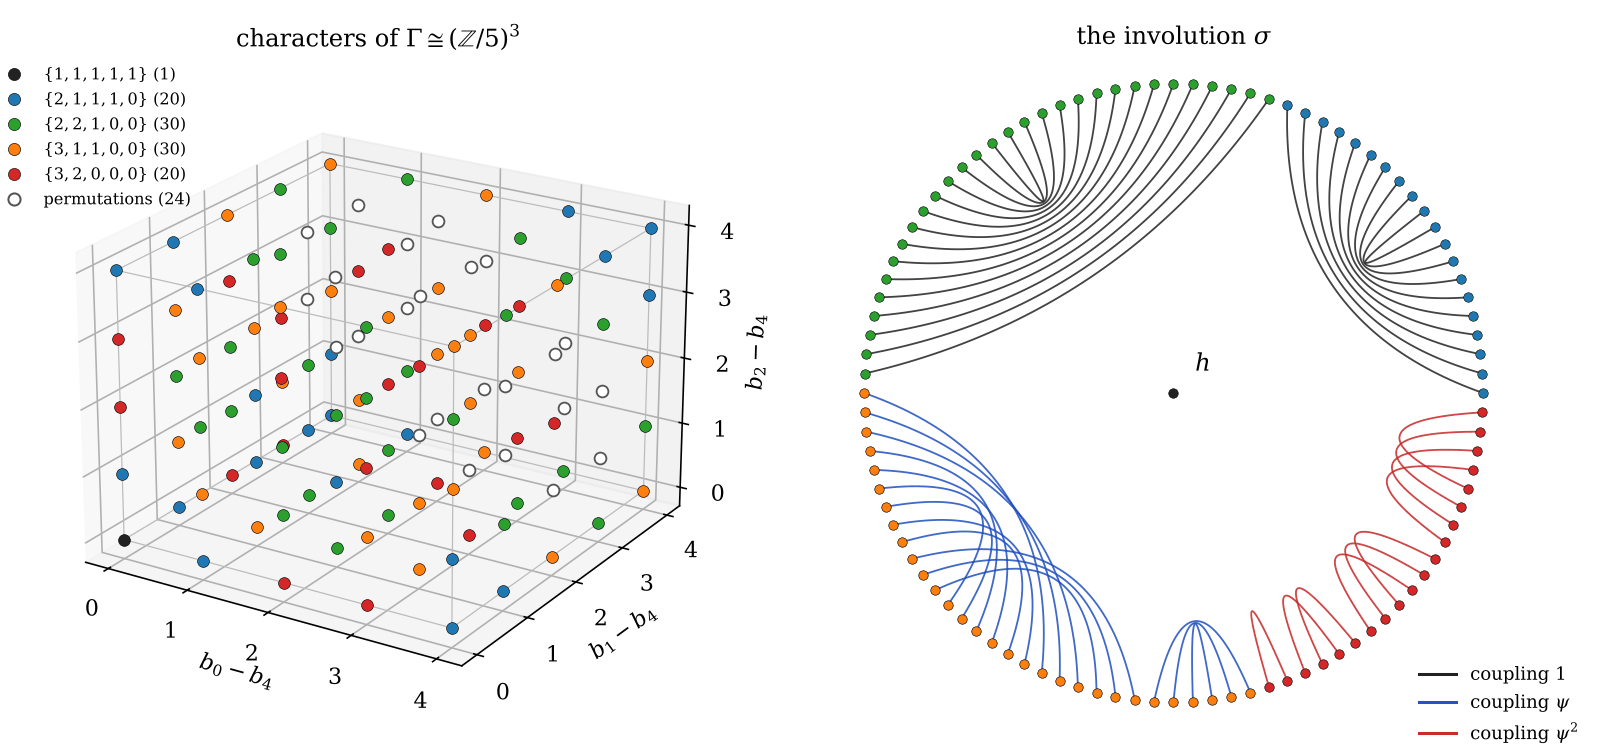
\includegraphics[width=0.96\textwidth]{figures/fig_labels.png}
\caption{The hundred and one generations of the Dwork quintic as points
of the character group of $\Gamma$. Left: $\widehat\Gamma\cong(\Z/5)^3$
drawn as a cube of $125$ points, the class of $\bb$ placed at
$(b_0-b_4,b_1-b_4,b_2-b_4)\bmod5$; the $101$ labels are filled and
coloured by type (the five $S_5$-orbits), and the $24$ classes of
permutations of $(0,1,2,3,4)$ are hollow. Right: the
involution $\sigma$ of Theorem~\ref{thm:C}, drawn as chords between paired
labels, with the chord colour giving the power of $\psi$ of the pairing:
black for $1$, blue for $\psi$, red for $\psi^2$; the fixed label is the
invariant class $h$ at the centre.}
\label{fig:labels}
\end{figure}

\section{The socle functional}\label{sec:socle}

Fix $\psi$ with $\psi^5\ne1$, write $R=R_{F_\psi}$ and $m_0=x_1^3x_2^3
x_3^3x_4^3x_5^3$, the only monomial of degree fifteen with all exponents at
most three. Define the sector of a monomial $x^{\ee}$ of degree fifteen as
follows: $\ee$ is in sector $r\in\{0,1,2,3,4\}$ if $e_i\equiv 3-r\pmod5$
for every $i$; otherwise $\ee$ is in no sector. Sector $4$ is empty, because
its exponents are at least four each.

\begin{theorem}[Socle functional]\label{thm:socle}
For $\psi^5\ne1$, $m_0\ne0$ in $R_{15}$, and the linear functional
$\lambda$ on $R_{15}$ with $\lambda(m_0)=1$ satisfies, for every monomial
$x^{\ee}$ of degree fifteen,
\[
\lambda(x^{\ee})=\begin{cases}\psi^{r}&\text{if $\ee$ is in sector $r$,}\\
0&\text{otherwise.}\end{cases}
\]
Moreover $\lambda(\Hess F_\psi)=3\,200\,000\,(1-\psi^5)$.
\end{theorem}

\begin{proof}
The relations $x_i^4\equiv\psi\prod_{j\ne i}x_j$ in $R$ give, for every
exponent vector $\ee$ with $e_i\ge4$,
\begin{equation}\label{eq:reduce}
x^{\ee}\equiv\psi\,x^{\ee'},\qquad \ee'=\ee+\one-5\,\ee_i,
\end{equation}
where $\ee_i$ is the $i$-th unit vector. If $\ee$ is in sector $r$ then
$\ee'$ is in sector $r-1$: its $i$-th entry is $e_i-4\equiv 3-(r-1)$ and the
other entries are $e_j+1\equiv3-(r-1)$. The sectors are listed by hand. In
sector $0$ the entries are congruent to $3$ and sum to fifteen, so they are
all equal to three and $\ee=(3,3,3,3,3)$. In sector $1$ the entries are congruent to
two, so each is $2$, $7$ or $12$; a twelve would leave three for four
entries of at least two, so the entries are $2$ or $7$, and a total of
fifteen forces exactly one seven: $\ee$ is a
permutation of $(7,2,2,2,2)$, and \eqref{eq:reduce} applied to the seven
gives $\psi\,m_0$. In sector $2$ the entries are $1$, $6$ or $11$, and the
total forces two sixes and three ones (an eleven would leave four for the
other four entries, which are congruent to one and so are all one, a total
of fifteen; but then $\ee=(11,1,1,1,1)$, and \eqref{eq:reduce} applied to
the eleven gives $(7,2,2,2,2)$, in sector $1$ as well). In sector $3$ the
entries are multiples of five, so $\ee$ is a permutation of $(15,0,0,0,0)$,
$(10,5,0,0,0)$ or $(5,5,5,0,0)$, and one reduction at an entry of at least
five lands in sector $2$. By induction on $r$, every monomial in sector $r$
satisfies $x^{\ee}\equiv\psi^rm_0$ in $R$.\footnote{The reduction
\eqref{eq:reduce} uses only the relation $\partial_iF_\psi/5=x_i^4-\psi
\prod_{j\ne i}x_j$. It lowers the $i$-th exponent by four and raises each of
the other four by one, so it preserves the degree and moves the class of
$\ee$ modulo $\one$ by $-5\ee_i+\one\equiv\one$; this is why the sectors,
which are the classes $(3-r)\one$, are permuted cyclically and why each
reduction costs exactly one factor of $\psi$.}

If $\ee$ is in no sector, the monomial $x^{\ee}$ has a nontrivial character
of $\Gamma$: its character is the class of $\ee$ modulo $\one$, which is
trivial exactly when $\ee\equiv c\one$ for some $c$, that is, when $\ee$ is
in a sector. The ideal $J_{F_\psi}$ is $\Gamma$-stable, so $R$ is graded by
the characters of $\Gamma$ and $x^{\ee}$ lies in a nontrivial isotypic
component of $R_{15}$. Since $R_{15}$ is one-dimensional it carries a single
character, and $m_0$ carries the trivial one; so if $m_0\ne0$, every
nontrivial component vanishes and $x^{\ee}\equiv0$.

It remains to show that $m_0\ne0$. The Hessian $\Hess F_\psi$ has degree
fifteen and is $\Gamma$-invariant, so its monomials in no sector vanish in
$R$ and the others are multiples of $m_0$:
$\Hess F_\psi\equiv H(\psi)\,m_0$, with $H(\psi)$ the sum over the sector
monomials of the Hessian of their coefficients times $\psi^r$. By
Macaulay's theorem $\Hess F_\psi\ne0$ in $R_{15}$, so $m_0\ne0$ and
$H(\psi)\ne0$. The Hessian matrix has diagonal entries $20x_i^3$ and
off-diagonal entries $-5\psi\prod_{k\ne i,j}x_k$, each of degree three; an
off-diagonal entry omits exactly the two coordinates of its row and column.
The determinant is the sum over permutations $\pi$ of the sign of $\pi$
times $\prod_i(\text{entry }(i,\pi(i)))$, and the monomial of $\pi$ depends
only on its cycle type: a fixed point $a$ contributes $x_a^3$ from the
diagonal and $x_a$ from every off-diagonal factor, and a moved coordinate
$m$ contributes $x_m$ from every off-diagonal factor whose row and column
both differ from $m$. Table~\ref{tab:hessian} lists the seven cycle types;
the derivation of each row is in Appendix~\ref{app:hessian}. Summing the
last column,
\begin{align*}
H(\psi)&=3\,200\,000-\big(2\,000\,000+1\,000\,000+375\,000\\
&\qquad+75\,000-187\,500-62\,500\big)\psi^5\\
&=3\,200\,000\,(1-\psi^5). \qedhere
\end{align*}
\end{proof}

\begin{table}[t]
\caption{The Hessian of $F_\psi$ in the socle, by cycle type of the
permutation. Each row gives the number of permutations, their sign, the
monomial they contribute, its sector $r$, and the total contribution to
$H(\psi)$ after the reduction $x^{\ee}\equiv\psi^rm_0$.}
\label{tab:hessian}
\centering
\begin{tabular}{lrrlrr}
\toprule
type & count & sign & monomial & $r$ & contribution\\
\midrule
$1^5$ & 1 & $+$ & $(3,3,3,3,3)$ & 0 & $3\,200\,000$\\
$2\,1^3$ & 10 & $-$ & $(5,5,5,0,0)$ & 3 & $-2\,000\,000\,\psi^5$\\
$3\,1^2$ & 20 & $+$ & $(6,6,1,1,1)$ & 2 & $-1\,000\,000\,\psi^5$\\
$4\,1$ & 30 & $-$ & $(7,2,2,2,2)$ & 1 & $-375\,000\,\psi^5$\\
$5$ & 24 & $+$ & $(3,3,3,3,3)$ & 0 & $-75\,000\,\psi^5$\\
$2^2\,1$ & 15 & $+$ & $(7,2,2,2,2)$ & 1 & $187\,500\,\psi^5$\\
$3\,2$ & 20 & $-$ & $(3,3,3,3,3)$ & 0 & $62\,500\,\psi^5$\\
\bottomrule
\end{tabular}
\end{table}

\begin{remark}[Normalisation]\label{rem:hessian}
With the residue normalisation $\lambda_{F}(\Hess F)=1$ of
\eqref{eq:jacobianyukawa}, the cubic form of the pencil is
$\lambda_{F_\psi}=\lambda/(3\,200\,000(1-\psi^5))$. For $\va=\bb=\cc=h$ the
monomial is $x^{3\one}=m_0$, so $Y(h,h,h)$ is a constant times
$1/(1-\psi^5)$, which is the coupling $5/(1-\psi^5)$ of~\cite{CDGP91} in
the gauge in which $\Omega$ is the residue of $\Omega_0/F_\psi$; the
factor five is the constant $c$ of \eqref{eq:jacobianyukawa} in that gauge.
All ratios of couplings at fixed $\psi$ are independent of these
constants, and Theorem~\ref{thm:B} is stated for $\lambda$.
\end{remark}

\section{Couplings}\label{sec:couplings}

\begin{proof}[Proof of Theorem~\ref{thm:B}]
By \eqref{eq:jacobianyukawa} and Theorem~\ref{thm:socle},
$Y(x^{\va},x^{\bb},x^{\cc})=\lambda(x^{\va+\bb+\cc})$ up to the
normalisation of Remark~\ref{rem:hessian}, and $\va+\bb+\cc$ has degree
fifteen; the value is $\psi^r$ if $\va+\bb+\cc\equiv(3-r)\one$ and zero
otherwise. For $\psi\ne0$ every sector value is nonzero. The count of the
unordered triples is in Section~\ref{sec:count}.
\end{proof}

\subsection{The count}\label{sec:count}

A triple $\{\va,\bb,\cc\}$ of elements of $B$, with repetitions allowed, has
a nonzero coupling exactly when $\va+\bb+\cc\equiv c\one\pmod5$ for some
$c$, and then $c\equiv3-r$ with $r$ the sector. We count ordered triples
first. The congruence says that the character of $\cc$ is the inverse of the
character of $\va+\bb$ in $\widehat\Gamma$. Every character occurs in $B$ at
most once (Theorem~\ref{thm:A}), so for each ordered pair $(\va,\bb)$ there
is at most one $\cc$, and there is one exactly when the class of
$-(\va+\bb)$ is one of the hundred and one realised classes, that is, when it
is not the class of a permutation of $(0,1,2,3,4)$. The negative of a
permutation of $(0,1,2,3,4)$ is, modulo five, a permutation of
$(0,1,2,3,4)$ again, so this fails exactly when $\va+\bb$ has five distinct
residues modulo five.

\emph{Excluded pairs.} The entries of $\va+\bb$ lie in $\{0,\dots,6\}$ and
sum to ten. Five distinct residues are the residues $0,1,2,3,4$, whose sum
is already ten, so no entry can exceed four and $\va+\bb$ is a permutation
of $(0,1,2,3,4)$. Fix the permutation, so that the coordinate $k$ of
$\va+\bb$ equals $k$ for $k=0,\dots,4$ after renaming. Write $p_k$ for the
part given to $\va$ in coordinate $k$; then $0\le p_k\le\min(k,3)$ and
$k-p_k\le3$, so $p_0=0$, $p_1\in\{0,1\}$, $p_2\in\{0,1,2\}$,
$p_3\in\{0,1,2,3\}$ and $p_4\in\{1,2,3\}$, and $|\va|=5$ means
$p_1+p_2+p_3+p_4=5$. The number of solutions is the coefficient of $t^5$ in
\[
(1+t)(1+t+t^2)(1+t+t^2+t^3)(t+t^2+t^3),
\]
which is $16$.\footnote{Expand $(1+t)(1+t+t^2)=1+2t+2t^2+t^3$ and
$(1+t+t^2+t^3)(t+t^2+t^3)=t+2t^2+3t^3+3t^4+2t^5+t^6$. The coefficient of
$t^5$ in the product is $1\cdot2+2\cdot3+2\cdot3+1\cdot2=16$, pairing the
terms of degree $0,1,2,3$ of the first factor with those of degree
$5,4,3,2$ of the second.} With $120$ permutations there are $1920$
excluded ordered pairs, so the number of ordered triples with a nonzero
coupling is $101^2-1920=8281$.

\emph{Repetitions.} An ordered triple $(\va,\va,\va)$ has a nonzero coupling
when $3\va\equiv c\one$, that is, when all entries of $\va$ are congruent
modulo five; entries in $\{0,1,2,3\}$ summing to five then force
$\va=\one$. For a triple $(\va,\va,\cc)$ the partner $\cc$ exists unless
$2\va$ has five distinct residues; the residues of $2a_i$ for
$a_i=0,1,2,3$ are $0,2,4,1$, and five distinct residues would need five
distinct entries of $\va$ in a set of four values, which is impossible. So
every $\va$ has a partner $\cc$, and $\cc=\va$ only for $\va=\one$. There
are therefore $100$ unordered triples of the form $\{\va,\va,\cc\}$ with
$\cc\ne\va$, giving $300$ ordered triples, one triple $\{\one,\one,\one\}$,
and $8281-300-1=7980$ ordered triples with three distinct entries. The
number of unordered triples is
\[
\frac{7980}{6}+100+1=1330+101=1431.
\]

\emph{Sectors.} In sector $r$ the sum $\ee=\va+\bb+\cc$ is one of the
vectors listed in the proof of Theorem~\ref{thm:socle} with entries at most
nine: $(3,3,3,3,3)$ for $r=0$, the five permutations of $(7,2,2,2,2)$ for
$r=1$, the ten permutations of $(6,6,1,1,1)$ for $r=2$ and the ten
permutations of $(5,5,5,0,0)$ for $r=3$. The number $O(\ee)$ of ordered
triples with sum $\ee$ is the coefficient of $x^5y^5$ in
$\prod_{i=1}^5P_{e_i}(x,y)$, where $P_e(x,y)=\sum x^ay^b$ over the pairs
$0\le a,b\le3$ with $0\le e-a-b\le3$. These coefficients are
\begin{gather*}
O(3,3,3,3,3)=3391,\quad O(7,2,2,2,2)=480,\\
O(6,6,1,1,1)=162,\quad O(5,5,5,0,0)=87,
\end{gather*}
so the ordered counts by sector are $3391$, $2400$, $1620$ and $870$, with
total $8281$. The hundred unordered triples $\{\va,\va,\cc\}$ with
$\cc\ne\va$ split as $0$, $50$, $20$ and $30$ by sector (the sector of
$2\va+\cc$), and $\{\one,\one,\one\}$ lies in sector $0$, so the unordered
counts are
\[
N_r=\frac{O_r-3D_r-T_r}{6}+D_r+T_r=566,\ 425,\ 280,\ 160,
\]
with $O_r$, $D_r$, $T_r$ the ordered, repeated and constant counts of
sector $r$. The coefficient extractions are written out in
Appendix~\ref{app:count}.

\section{The mass map}\label{sec:mass}

\begin{proof}[Proof of Theorem~\ref{thm:C}]
For $\bb\in B$ the coupling $\lambda(x^{\bb+\cc+\one})$ is nonzero exactly
when $\bb+\cc+\one\equiv(3-r)\one$, that is $\cc\equiv(2-r)\one-\bb\pmod5$,
with $\cc\in B$. For each $r$ the residues of $(2-r)\one-\bb$ are
determined, and $\cc$ exists in $B$ exactly when those residues, taken in
$\{0,1,2,3\}$ (a residue $4$ excludes), sum to five. Go through the types.
If all $b_i\le2$ then $r=0$ gives $\cc=2\one-\bb\in\{0,1,2\}^5$ of sum five:
this is the partner. For $r=1$ the residues of $\one-\bb$ are $1,0,4$ for
$b_i=0,1,2$, so a two in $\bb$ excludes, and $\bb\in\{0,1\}^5$ of sum five
means $\bb=\one$, whose $r=1$ residues are all zero, sum zero: excluded. For
$r=2$ the residues of $-\bb$ are $0,4,3$: a one excludes, and $\bb\in\{0,2\}^5$
has even sum: excluded. For $r=3$ the residues of $-\one-\bb$ are $4,3,2$: a
zero excludes, so $\bb\in\{1,2\}^5$ of sum five means $\bb=\one$, residues
all $3$, sum fifteen: excluded. So a label with entries at most two has
exactly one partner, $2\one-\bb$, with coupling $1$; this covers the
fifty-one labels of the types $\{1,1,1,1,1\}$, $\{2,1,1,1,0\}$ and
$\{2,2,1,0,0\}$, and $\sigma(\bb)=2\one-\bb$ is of the same type, with the
single fixed point $\bb=\one$.

If $\bb$ has type $\{3,1,1,0,0\}$: $r=0$ gives residue $4$ at the three,
excluded; $r=1$ gives residues $3,0,0,1,1$, sum five, so $\cc$ is the label
with $3$ where $\bb$ has $3$, zeros where $\bb$ has ones and ones where
$\bb$ has zeros, of the same type, with coupling $\psi$; $r=2$ gives
residues $2,4,\dots$, excluded by the ones; $r=3$ gives residues $1,3,3,4,4$,
excluded. If $\bb$ has type $\{3,2,0,0,0\}$: $r=0$ excluded by the three;
$r=1$ gives residues $3,4,\dots$, excluded by the two; $r=2$ gives residues
$2,3,0,0,0$, sum five, so $\cc$ swaps the three and the two of $\bb$, of the
same type, coupling $\psi^2$; $r=3$ gives residues $1,2,4,4,4$, excluded.
This proves that every label has exactly one partner, that
$\sigma$ is an involution preserving type with the one fixed point $\one$,
and the three values of the coupling. The matrix $M=(\lambda(x^{\bb+\cc+
\one}))_{\bb,\cc}$ is therefore a monomial matrix with entries $1$ (fifty-one
times), $\psi$ (thirty times) and $\psi^2$ (twenty times), so its
determinant is $\psi^{30+40}=\psi^{70}$, the sign of $\sigma$, a product of
fifty transpositions, being $+1$, and its rank is $101$ for
$\psi\ne0$. At $\psi=0$ the rows of the fifty labels containing a three
vanish and the remaining fifty-one rows are a permutation matrix on the
fifty-one labels with entries at most two: rank fifty-one.

The $\Gamma$-invariant Hermitian metric on $H^{2,1}$, the Hodge metric,
pairs the isotypic components of distinct characters to zero because a
unitary representation of a finite abelian group is an orthogonal sum of its
isotypic components; by Theorem~\ref{thm:A} the components are the lines
spanned by the $x^{\bb}$, so the metric is diagonal with entries $g_{\bb}$.
The mass matrix \eqref{eq:massmatrix} is then $v$ times a monomial matrix
with entries $\psi^{r(\bb)}(g_{\bb}g_{\sigma\bb})^{-1/2}$ at $(\bb,\sigma
\bb)$. The singular values of a symmetric monomial matrix with an
involution are the absolute values of its entries, each two-cycle giving a
doubly degenerate pair and the fixed point a singlet; this is the stated
spectrum.
\end{proof}

\begin{figure}[t]
\centering
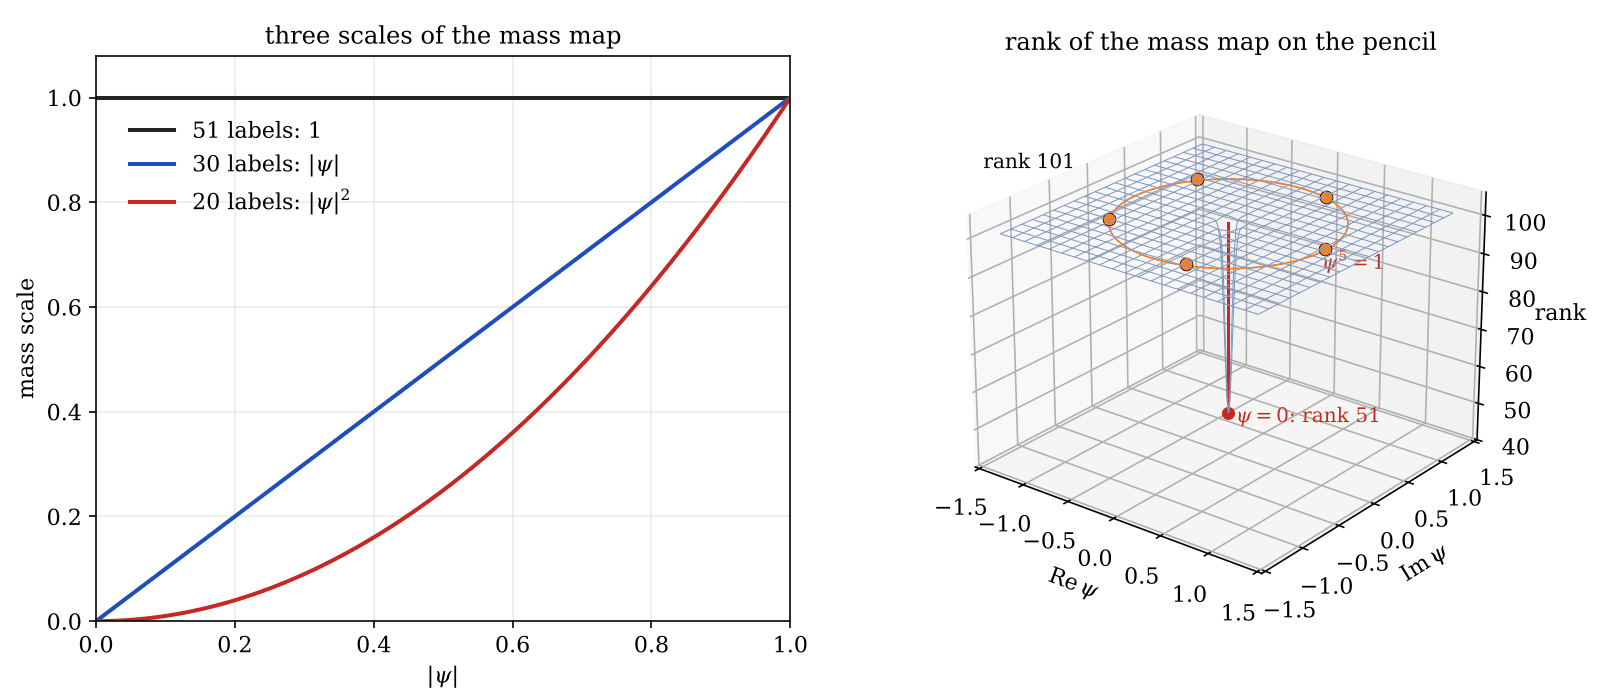
\includegraphics[width=0.96\textwidth]{figures/fig_masses.png}
\caption{The mass spectrum of Theorem~\ref{thm:C} along the pencil. Left:
the three mass scales $1$, $|\psi|$ and $|\psi|^2$ against $|\psi|$ for
$0\le|\psi|<1$, with the multiplicities of the labels (fifty-one, thirty,
twenty) that carry them; the singlet $h$ sits in the first group. Right: the
rank of the mass map over the $\psi$-plane, fifty-one at the Fermat point
and a hundred and one elsewhere (the drop at $\psi=0$ is drawn with a small
width); the conifold points $\psi^5=1$, where the Jacobian ring
degenerates, are marked on the unit circle.}
\label{fig:masses}
\end{figure}

\begin{remark}[Degenerations]
The determinant $\pm\psi^{70}$ shows that the mass map of the invariant
direction degenerates on the pencil only at the Fermat point, where the
group of automorphisms of $X_\psi$ jumps from $\Gamma\rtimes S_5$ to the
full group of order $5^4\cdot120$ of the Fermat quintic. The fifty massless
generations at $\psi=0$ are the labels with an exponent three. The larger
group acts on a monomial through its full exponent vector, not only through
its class modulo $\one$, so at $\psi=0$ a coupling of $h$, $\bb$ and $\cc$
survives only if $\one+\bb+\cc=(3,3,3,3,3)$; for a label with an exponent
three the required partner $2\one-\bb$ has a negative entry.
At the conifold points $\psi^5=1$ the matrix $M$ has nonzero determinant,
but the normalisation of Remark~\ref{rem:hessian} has a pole: the physical
couplings diverge as $1/(1-\psi^5)$ in the gauge of $\Omega$ chosen there,
and the Hodge norm of $h$ diverges logarithmically, as in~\cite{CDGP91}.
\end{remark}

\section{The Fermat point}\label{sec:fermat}

At $\psi=0$ the Hodge norms are explicit.

\begin{proposition}[Hodge norms at the Fermat point]\label{prop:fermat}
Let $X_0$ be the Fermat quintic and $\omega_{\bb}$ the class of $x^{\bb}$,
$\bb\in B$. Write $k_i=b_i+1$ and $\gamma(t)=\Gamma(t)/\Gamma(1-t)$. There
is a constant $C>0$ independent of $\bb$ such that
\begin{equation}\label{eq:gamma}
g_{\bb}=\ip{\omega_{\bb}}{\overline{\omega_{\bb}}}=C\prod_{i=1}^5
\gamma(k_i/5).
\end{equation}
\end{proposition}

\begin{proof}
The full group $\mu_5^5/\mu_5$ of diagonal phases acts on $X_0$, and
$\omega_{\bb}$ spans the eigenline of the character $\mathbf k=(k_i)$, with
$1\le k_i\le4$ and $\sum k_i=10$. Eigenlines of distinct characters are
orthogonal for the Hodge metric, so $g_{\bb}$ is the only entry of the
metric on that line, and it is computed from the periods of $\omega_{\bb}$
by the second Riemann bilinear relation: if $P$ is an integral cycle and
$P_{\mathbf k}$ its component in the eigenspace of $\mathbf k$ in
$H_3(X_0,\C)$, then $g_{\bb}=|\int_P\omega_{\bb}|^2/
|P_{\mathbf k}\cdot P_{-\mathbf k}|$ up to a factor depending only on the
Hodge type. For the cycle of Pham, the join of the five sets of fifth roots
of unity, the period is a product of beta integrals, and the intersection
number is a product of factors $1-\zeta^{k_i}$; combining them with
$\Gamma(t)\Gamma(1-t)=\pi/\sin\pi t$ gives \eqref{eq:gamma}. This is the
computation of Candelas~\cite{Can88} on the Fermat quintic and, in the
language of the Gepner model, of Distler and Greene~\cite{DG88}; the steps
are written out in Appendix~\ref{app:fermat}.
\end{proof}

The proposition fixes the ratios of the Hodge norms inside $H^{2,1}$, which
is all that the masses of Theorem~\ref{thm:C} need. Since $\gamma(1-t)=
1/\gamma(t)$, every norm is a monomial in the two numbers
$\gamma(1/5)=3.94325$ and $\gamma(2/5)=1.48951$. For the singlet,
$\mathbf k=(2,2,2,2,2)$ and $g_{\one}=C\gamma(2/5)^5$; for the type
$\{2,1,1,1,0\}$, $\mathbf k$ is a permutation of $(3,2,2,2,1)$ and
$g_{\bb}=C\gamma(2/5)^2\gamma(1/5)$; for the type $\{2,2,1,0,0\}$,
$\mathbf k$ is a permutation of $(3,3,2,1,1)$ and $g_{\bb}=C\gamma(1/5)^2/
\gamma(2/5)$. The ratio of the second to the first is
$\Gamma(3/5)^3\Gamma(1/5)/\Gamma(2/5)^3\Gamma(4/5)=1.19324$, the square of
the constant $\kappa=1.09236$ in which Distler and Greene~\cite{DG88}
expressed the normalised couplings of the Gepner model
(see~\cite[eq.~(4.3)]{BMT24}). The norm of $\Omega$, the class of $1$ with
$\mathbf k=(1,1,1,1,1)$, has the same shape with a different constant, and
the Weil--Petersson metric of the pencil at the Fermat point, computed from
the periods by Candelas, de la Ossa, Green and Parkes~\cite{CDGP91}, is
\[
G_{\psi\bar\psi}(0)=25\,\frac{\Gamma(2/5)^5\,\Gamma(4/5)^5}
{\Gamma(1/5)^5\,\Gamma(3/5)^5}=0.19226,
\]
the value that Butbaia and collaborators~\cite{BMT24} reproduce with
numerical Ricci-flat metrics.\footnote{In~\cite{BMT24} the value is given
for the mirror quintic, whose complex structure moduli space is the
$\psi$-line of the Dwork pencil divided by the symmetry
$\psi\mapsto\zeta\psi$. The Weil--Petersson metric is
$-\partial\bar\partial\log\int\Omega\wedge\overline\Omega$, and passing to
the quotient by $\Gamma$ multiplies $\int\Omega\wedge\overline\Omega$ by the
constant $1/125$, which does not change the metric; the two numbers are
therefore the same. Their machine-learned harmonic representatives give
$0.1906$ against the exact $0.1923$.}

Inserting \eqref{eq:gamma} into Theorem~\ref{thm:C} gives the fifty-one
nonzero masses at the Fermat point. Each label of the types
$\{2,1,1,1,0\}$ and $\{2,2,1,0,0\}$ is paired with a label of the same type
and the same multiset of $k_i$, so $g_{\bb}=g_{\sigma\bb}$ and its mass is
$v/g_{\bb}$; the singlet has mass $v/g_{\one}$. Table~\ref{tab:fermat} lists
the values. In units of the singlet mass the two doublet masses are
$0.83805$ (twenty labels, ten doublets) and $0.70234$ (thirty labels,
fifteen doublets). The fifty generations with an exponent three are
massless there, and acquire masses proportional to $|\psi|$ (thirty) and
$|\psi|^2$ (twenty) as the modulus moves off the Fermat point.

\begin{table}[t]
\caption{Hodge norms and masses at the Fermat point, from
\eqref{eq:gamma} and Theorem~\ref{thm:C}. Norms are in units of $C$ and
masses in units of $v/C$; the types with an exponent three are massless at
$\psi=0$.}
\label{tab:fermat}
\centering
\begin{tabular}{lrlll}
\toprule
type & count & $g_{\bb}/C$ & value & mass\\
\midrule
$\{1,1,1,1,1\}$ & 1 & $\gamma(2/5)^5$ & $7.33179$ & $0.136392$\\
$\{2,1,1,1,0\}$ & 20 & $\gamma(2/5)^2\gamma(1/5)$ & $8.74859$ & $0.114304$\\
$\{2,2,1,0,0\}$ & 30 & $\gamma(1/5)^2/\gamma(2/5)$ & $10.4392$ & $0.095793$\\
$\{3,1,1,0,0\}$ & 30 & $\gamma(2/5)^2\gamma(1/5)$ & $8.74859$ & $0$\\
$\{3,2,0,0,0\}$ & 20 & $\gamma(1/5)^2/\gamma(2/5)$ & $10.4392$ & $0$\\
\bottomrule
\end{tabular}
\end{table}

\section{Weighted Fermat pencils}\label{sec:weighted}

\subsection{The pencils}

In this section $(d;w)$ is one of $(6;1,1,1,1,2)$, $(8;1,1,1,1,4)$ and
$(10;1,1,1,2,5)$, so that $d=\sum w_i$ and $n_i=d/w_i$ is an integer:
$n=(6,6,6,6,3)$, $(8,8,8,8,2)$ and $(10,10,10,5,2)$. The polynomial
$F_\psi=\sum_ix_i^{n_i}-d\psi P$, $P=x_1x_2x_3x_4x_5$, is weighted
homogeneous of degree $d$ for $\deg x_i=w_i$, and $X_\psi\subset\PP(w)$ is
its zero locus \eqref{eq:wpencil}. We write
\[
\delta=\prod_iw_i^{w_i}\in\{4,\,256,\,12\,500\},
\]
and use the letters $i,j,k,l$ for distinct indices among the coordinates of
weight one. Table~\ref{tab:wdata} collects the numbers proved in this
section, with the quintic for comparison.\footnote{The three pencils are the
weighted members of the family of one-parameter models whose periods and
mirror maps were computed by Morrison~\cite{Mor92}, Klemm and
Theisen~\cite{KT93} and Font~\cite{Fon93}. In those papers the coefficient
of $P$ is normalised differently and the natural coordinate on the moduli
space is $\psi^d$ up to a constant; the discriminant $\psi^d\delta=1$ below
is the conifold locus of those papers, and the Fermat point $\psi=0$ is the
Gepner point.}

\begin{table}[t]
\caption{The four pencils of Fermat type. The rows give the degree and
weights, the constant $\delta=\prod w_i^{w_i}$ of the discriminant
$\psi^d\delta=1$, the intersection numbers of the hyperplane class $L$, the
Euler characteristic and $h^{2,1}$, the order of $\Gamma$, the number of
distinct characters carried by the generations, the number of classes of
two or three generations sharing a character, the number of characters of
$\Gamma$ carried by no generation, and the rank of the mass map of the
invariant direction for $\psi\ne0$ and at $\psi=0$, with the number of
generations it leaves massless.}
\label{tab:wdata}
\centering
\begin{tabular}{lcccc}
\toprule
 & quintic & sextic & octic & dectic\\
\midrule
$(d;w)$ & $(5;1,1,1,1,1)$ & $(6;1,1,1,1,2)$ & $(8;1,1,1,1,4)$ & $(10;1,1,1,2,5)$\\
$\delta$ & $1$ & $4$ & $256$ & $12\,500$\\
$L^3$, $c_2\cdot L$ & $5$, $50$ & $3$, $42$ & $2$, $44$ & $1$, $34$\\
$\chi$, $h^{2,1}$ & $-200$, $101$ & $-204$, $103$ & $-296$, $149$ & $-288$, $145$\\
$|\Gamma|$ & $125$ & $108$ & $128$ & $100$\\
distinct characters & $101$ & $96$ & $122$ & $100$\\
shared classes & $0$ & $7$ & $27$ & $42$\\
characters not carried & $24$ & $12$ & $6$ & $0$\\
rank for $\psi\ne0$ (massless) & $101$ ($0$) & $99$ ($4$) & $125$ ($24$) & $109$ ($36$)\\
rank at $\psi=0$ (massless) & $51$ ($50$) & $44$ ($59$) & $85$ ($64$) & $72$ ($73$)\\
\bottomrule
\end{tabular}
\end{table}

\begin{lemma}\label{lem:wsmooth}
If $\psi^d\delta\ne1$, then $X_\psi$ is quasi-smooth, it misses the singular
points of $\PP(w)$, and it is a smooth Calabi--Yau threefold with
$h^{1,1}=1$. Its hyperplane class $L=c_1(\cO_X(1))$ generates $H^2(X,\Z)$
modulo torsion, and
\begin{equation}\label{eq:wchern}
\begin{gathered}
L^3=\frac{d}{\prod_iw_i},\qquad c_2\cdot L=\sigma_2(w)\,L^3,\\
\chi=\big(\sigma_3(w)-d\,\sigma_2(w)\big)L^3,
\end{gathered}
\end{equation}
with $\sigma_k$ the elementary symmetric functions of the weights. If
$\psi^d\delta=1$, then $X_\psi$ is singular.
\end{lemma}

\begin{proof}
The Euler relations $x_i\partial_iF_\psi=n_ix_i^{n_i}-d\psi P$ show that at a
common zero of the partial derivatives $x_i^{n_i}=w_i\psi P$ for every $i$.
If $P=0$ this forces $x=0$. Otherwise raise the $i$-th relation to the power
$w_i$ and multiply: since $\prod_ix_i^{n_iw_i}=P^d$, this gives
$P^d=\psi^d\delta P^d$, so $\psi^d\delta=1$. Hence $X_\psi$ is quasi-smooth
when $\psi^d\delta\ne1$. Conversely, at $\psi=2^{-1/3}$, $\psi=1/2$ and
$\psi=2^{-1/5}5^{-1/2}$ the points $(1,1,1,1,2^{1/3})$, $(1,1,1,1,2)$ and
$(1,1,1,2^{1/5},5^{1/2})$ satisfy $x_i^{n_i}=w_i\psi P=w_i$, so they are
singular points of the sextic, octic and dectic; the other roots of
$\psi^d\delta=1$ are $\zeta\psi$ with $\zeta^d=1$, and
$x_1\mapsto\zeta^{-1}x_1$ maps $X_{\zeta\psi}$ to $X_\psi$ because $n_1=d$.

The singular points of $\PP(w)$ are $(0{:}0{:}0{:}0{:}1)$ for the sextic
and the octic, with isotropy $\mu_2$ and $\mu_4$, and $(0{:}0{:}0{:}1{:}0)$
and $(0{:}0{:}0{:}0{:}1)$ for the dectic, with isotropy $\mu_2$ and $\mu_5$.
Each monomial $x_i^{n_i}$ occurs in $F_\psi$ with coefficient one, so $F_\psi$
does not vanish at a coordinate point and $X_\psi$ misses them all; a
quasi-smooth hypersurface in the smooth locus of $\PP(w)$ is smooth. By
adjunction $K_X=\cO_X(d-\sum w_i)=\cO_X$, and the Lefschetz theorem for
quasi-smooth hypersurfaces~\cite{Dol82} gives $h^{1,0}=h^{2,0}=0$ and
$h^{1,1}=1$.

The tangent bundle of $\PP(w)$ on its smooth locus has total Chern class
$\prod_i(1+w_iH)$ by the weighted Euler sequence, and the normal bundle of
$X$ is $\cO_X(d)$, so $c(T_X)=\prod_i(1+w_iL)(1+dL)^{-1}$. Expanding with
$\sigma_1(w)=d$ gives $c_1=0$, $c_2=\sigma_2L^2$ and
$c_3=(\sigma_3-d\sigma_2)L^3$, and $L^3=d\int_{\PP(w)}H^4=d/\prod w_i$. For
the three pencils $(\sigma_2,\sigma_3)=(14,16)$, $(22,28)$ and $(34,52)$,
which gives Table~\ref{tab:wdata}. If $L=mL'$ with $L'$ integral, then
$m^3$ divides $L^3\in\{3,2,1\}$, which is cube-free, so $m=\pm1$; as
$H^2(X,\Q)$ is spanned by $L$, the class $L$ generates $H^2(X,\Z)$ modulo
torsion.
\end{proof}

\subsection{Labels and characters}

The Jacobian ring $R=\C[x_1,\dots,x_5]/(\partial_1F_\psi,\dots,
\partial_5F_\psi)$ is graded by $\deg x_i=w_i$. Quasi-smoothness says that
the partial derivatives, of degrees $d-w_i$, form a regular sequence, so
$R$ is a graded complete intersection with Hilbert series
$\prod_i(1-t^{d-w_i})/(1-t^{w_i})$: it has dimension $\prod_i(n_i-1)$, which
is $1250$, $2401$ and $2916$, its top degree is $\sum_i(d-2w_i)=3d$, and
$R_{3d}$ is one-dimensional and spanned by $\Hess F_\psi$ by Macaulay's
theorem, which holds for any regular sequence of weighted homogeneous
polynomials. Griffiths' description of the Hodge structure extends to
quasi-smooth hypersurfaces in weighted projective space, as shown by
Steenbrink~\cite{Ste77} and Dolgachev~\cite{Dol82}: with
\[
\Omega_0=\sum_i(-1)^iw_ix_i\,dx_1\wedge\cdots\widehat{dx_i}\cdots\wedge dx_5,
\]
the residue along $X$ of $P\,\Omega_0/F_\psi^{q+1}$, for $P$ of degree
$qd$, identifies $R_{qd}$ with $H^{3-q,q}(X)$, so that $H^{2,1}=R_d$ and
$R_{3d}$ is the socle. The
infinitesimal variation of the Hodge structure is again multiplication in
$R$, and the cubic form is \eqref{eq:jacobianyukawa} with $\lambda$ a
functional on $R_{3d}$; the derivation in~\cite{CG80} uses only the residue
map and the residue pairing of $R$, both of which are available in the
weighted setting.

Let $B$ be the set of $\bb\in\Z^5$ with $0\le b_i\le n_i-2$ and
$\sum_iw_ib_i=d$. We call its elements the labels.

\begin{lemma}\label{lem:wlabels}
Let $\psi^d\delta\ne1$. Every monomial $x^{\ee}$ of degree $d$ satisfies
$x^{\ee}\equiv c\,\psi^r x^{\bb}$ in $R$ with $\bb\in B$, $c$ a product of
weights, and $r\le1$ for the sextic and $r\le2$ for the octic and the
dectic. The monomials $x^{\bb}$, $\bb\in B$, are a basis of $R_d=H^{2,1}$,
so $|B|=h^{2,1}$.
\end{lemma}

\begin{proof}
The relations $\partial_iF_\psi/n_i=0$ read
\begin{equation}\label{eq:wreduce}
x_i^{n_i-1}\equiv w_i\psi\prod_{j\ne i}x_j .
\end{equation}
In a monomial of degree $d$ at most one exponent satisfies $e_i\ge n_i-1$:
two such exponents would carry weight at least $2d-w_i-w_j>d$. If
$e_i\ge n_i-1$, then $e_i\in\{n_i-1,n_i\}$, and \eqref{eq:wreduce} replaces
$x^{\ee}$ by $w_i\psi\,x^{\ee'}$ with $e'_i=e_i-n_i+1$ and $e'_j=e_j+1$ for
$j\ne i$. If $e_i=n_i$, then $x^{\ee}=x_i^{n_i}$ and $\ee'=\one$. If
$e_i=n_i-1$, then $e'_i=0$, the other coordinates carry weight $w_i$, and
$e'_j\ge n_j-1$ forces $w_je_j\ge d-2w_j$, hence $w_i+2w_j\ge d$. For the
sextic no pair $i\ne j$ has $w_i+2w_j\ge6$, and $\one\in B$ because every
$n_j\ge3$; so one step suffices. For the octic and the dectic the only $j$
with $w_i+2w_j\ge d$ for some $i\ne j$ is $j=5$, where $w_5=d/2$ and
$n_5=2$; in that case, and in the case $\ee'=\one$, the exponent of $x_5$
is one and a second step at $x_5$ gives an exponent vector with $e''_5=0$
and the other entries raised by one. A third step would need $w_5+2w_k\ge
d$, that is $w_k\ge d/4$, for some $k\le4$, which fails. So at most two
steps reach a vector with all $e_i\le n_i-2$, which is a label.

At $\psi=0$ the ring is $\bigotimes_i\C[x_i]/(x_i^{n_i-1})$, whose
monomials with $e_i\le n_i-2$ are a basis; so $|B|=\dim R_d$. The Hilbert
series does not depend on $\psi$, and the labels span $R_d$ for every
$\psi$ by the first part, so they are a basis.
\end{proof}

\paragraph*{The symmetry group.}
Let $K$ be the group of $\varepsilon\in\prod_i\mu_{n_i}$ with
$\prod_i\varepsilon_i=1$, acting by $x_i\mapsto\varepsilon_ix_i$. It
preserves $F_\psi$ for every $\psi$. The elements
$(\lambda^{w_1},\dots,\lambda^{w_5})$ with $\lambda^d=1$ lie in $K$ and act
trivially on $\PP(w)$, and they are the only such elements; they form a
subgroup isomorphic to $\mu_d$ because the weights are coprime. Let
$\Gamma=K/\mu_d$. Since $\mathrm{lcm}(n_i)=d$, the product map
$\prod_i\mu_{n_i}\to\mu_d$ is onto and $|\Gamma|=\prod_in_i/d^2$, which is
$108$, $128$ and $100$. A character of $\prod_i\mu_{n_i}$ is a vector
$\bb\in\bigoplus_i\Z/n_i$, acting by $\varepsilon\mapsto\prod_i
\varepsilon_i^{b_i}$; it is trivial on $K$ exactly when it is a multiple of
$\one$, and it is trivial on $\mu_d$ exactly when $\sum_iw_ib_i\equiv0
\pmod d$, a condition that is well defined because $w_in_i=d$. Hence
\[
\widehat\Gamma=\Big\{\bb\in\textstyle\bigoplus_i\Z/n_i:\ \sum_iw_ib_i
\equiv0\pmod d\Big\}\Big/\langle\one\rangle .
\]
A monomial $x^{\ee}$ of degree divisible by $d$ transforms by the class
$[\ee]$ of its exponent vector, and $\Omega_0$ transforms by
$\prod_i\varepsilon_i=1$, so the isomorphisms $R_{qd}\cong H^{3-q,q}$ are
$\Gamma$-equivariant and $R$ is graded by $\widehat\Gamma$. The Hessian is
invariant, since $\partial_i\partial_jF_\psi$ transforms by
$\varepsilon_i^{-1}\varepsilon_j^{-1}$ and the determinant by
$\prod_i\varepsilon_i^{-2}=1$; so $R_{3d}$ carries the trivial character.
Permutations of coordinates of equal weight also preserve $F_\psi$ and
permute the labels.

\begin{lemma}[Wrapping]\label{lem:wwrap}
Two labels $\bb\ne\bb'$ carry the same character if and only if there is a
shift $s\in\{1,\dots,d-1\}$ such that, with $a_i=\lfloor(b_i+s)/n_i\rfloor$,
\[
\begin{gathered}
b'_i=b_i+s-n_ia_i,\qquad \sum_ia_i=s,\\
b_i+s\not\equiv n_i-1\pmod{n_i}\quad\text{for all }i .
\end{gathered}
\]
The shift from $\bb'$ back to $\bb$ is then $d-s$.
\end{lemma}

\begin{proof}
Both labels satisfy $\sum w_ib_i=d\equiv0$, so they define the same
character exactly when $\bb'\equiv\bb+s\one$ modulo $(n_1,\dots,n_5)$ for
some $s$ modulo $d$. As $0\le b'_i\le n_i-2$, the entry $b'_i$ is the
residue of $b_i+s$ in $\{0,\dots,n_i-1\}$, which must differ from $n_i-1$.
Then $\sum_iw_ib'_i=\sum_iw_ib_i+sd-d\sum_ia_i$, which equals $d$ exactly
when $\sum_ia_i=s$.
\end{proof}

\begin{proposition}\label{prop:wchars}
Let $\psi^d\delta\ne1$. The classes of labels that carry the same character
are exactly the following, and every other label carries a character of its
own.
\begin{enumerate}[label=\textup{(\alph*)},leftmargin=*,itemsep=1pt]
\item Sextic: the $4$ pairs $\{x_i^4x_5,\ x_j^2x_k^2x_l^2\}$ at shift
$2$ and the $3$ pairs $\{x_i^3x_j^3,\ x_k^3x_l^3\}$ at shift $3$; $96$
distinct characters.
\item Octic: the $12$ pairs $\{x_i^6x_j^2,\ x_j^4x_k^2x_l^2\}$ and the $12$
pairs $\{x_i^6x_jx_k,\ x_j^3x_k^3x_l^2\}$ at shift $2$, and the $3$ pairs
$\{x_i^4x_j^4,\ x_k^4x_l^4\}$ at shift $4$; $122$ distinct characters.
\item Dectic: the $3$ triples $\{x_i^8x_4,\ x_j^2x_k^2x_4^3,\
x_i^2x_j^4x_k^4\}$; at shift $2$ the $12$ pairs $\{x_1^{c_1}x_2^{c_2}
x_3^{c_3}x_4^3,\ x_1^{c_1+2}x_2^{c_2+2}x_3^{c_3+2}\}$ with $c_1+c_2+c_3=4$
and $\cc$ not a permutation of $(2,2,0)$, the $6$ pairs
$\{x_i^8x_j^2,\ x_j^4x_k^2x_4^2\}$ and the $3$ pairs
$\{x_i^8x_jx_k,\ x_j^3x_k^3x_4^2\}$; at shift $4$ the $6$ pairs
$\{x_i^6x_j^2x_4,\ x_j^6x_k^4\}$, the $3$ pairs
$\{x_i^6x_jx_kx_4,\ x_j^5x_k^5\}$, the $6$ pairs
$\{x_i^7x_jx_4,\ x_ix_j^5x_k^4\}$ and the $3$ pairs
$\{x_i^6x_4^2,\ x_j^4x_k^4x_4\}$; $100$ distinct characters, so every
character of $\Gamma$ is carried by some generation.
\end{enumerate}
The characters carried by no label are the $12$ classes of
$(\pi(0,1,3,4),2)$ for the sextic and the $6$ classes of
$(\pi(0,2,4,6),1)$ for the octic, $\pi$ running over the permutations of
four entries. The set of characters carried by labels is closed under
$\chi\mapsto-\chi$.
\end{proposition}

\begin{proof}
We use Lemma~\ref{lem:wwrap} and treat the shifts $s\le d/2$; the others
are their inverses. For the sextic, $b_i+s\le9<12$ for $i\le4$, so
$a_i=1$ exactly when $b_i\ge6-s$, and the residue $n_i-1=5$ is excluded
when $b_i=5-s$; for $x_5$, $b_5\le1$ and $a_5=\lfloor(b_5+s)/3\rfloor$,
with $b_5+s\equiv2\pmod3$ excluded. At $s=1$ we have $a_5=0$ and need one
$b_i\ge5$, which is impossible. At $s=2$ the value $b_5=0$ is excluded, so
$b_5=1$ and $a_5=1$; we need exactly one $b_i\ge4$ among the first four,
which sum to four, so $\bb=(4,0,0,0,1)$ up to order, and its image is
$(0,2,2,2,0)$. At $s=3$ we have $a_5=1$ and need two entries $b_i\ge3$
among the first four and none equal to two; two entries of at least three
already have weight six, so $\bb=(3,3,0,0,0)$ up to order, with image
$(0,0,3,3,0)$. No label occurs at two different shifts, so the classes are
the pairs listed, $14$ labels in $7$ classes and $103-7=96$ characters.
The same analysis for the octic and the dectic is carried out in
Appendix~\ref{app:wlabels}. It uses two facts: for these pencils $n_5=2$
and $b_5=0$, so $a_5=s/2$ and an odd shift is excluded by the residue of
$x_5$; and the bounds $b_i\le n_i-2$ make each $a_i$ either $0$ or $1$,
except $a_4\in\{0,1,2\}$ for the dectic.

The characters not carried by a label are $108-96=12$, $128-122=6$ and
$100-100=0$ in number. For the sextic, adding $s\one$ to
$(\pi(0,1,3,4),2)$ gives a vector with an entry $5$ for $s\not\equiv0
\pmod3$, and the vector $(\pi'(0,1,3,4),2)$ for $s=3$, where the last entry
is $n_5-1$. So every representative of these classes has an entry $n_i-1$,
and none is a label; each class contains two of the $24$ vectors
$(\pi(0,1,3,4),2)$, which gives $12$ classes, and these are all the missing
characters. For the octic, adding $s\one$ to $(\pi(0,2,4,6),1)$ gives an
entry $7$ when $s$ is odd and the last entry $1=n_5-1$ when $s$ is even;
each class contains four of the $24$ vectors, which gives $6$ classes.
Finally $-(\pi(0,1,3,4),2)=(\pi(0,5,3,2),1)$, which becomes
$(\pi(1,0,4,3),2)$ after adding $\one$, and $-(\pi(0,2,4,6),1)=
(\pi(0,6,4,2),1)$; so the missing characters are closed under negation,
and so are the carried ones.
\end{proof}

Figure~\ref{fig:weighted} compares the four pencils.

\begin{figure}[t]
\centering
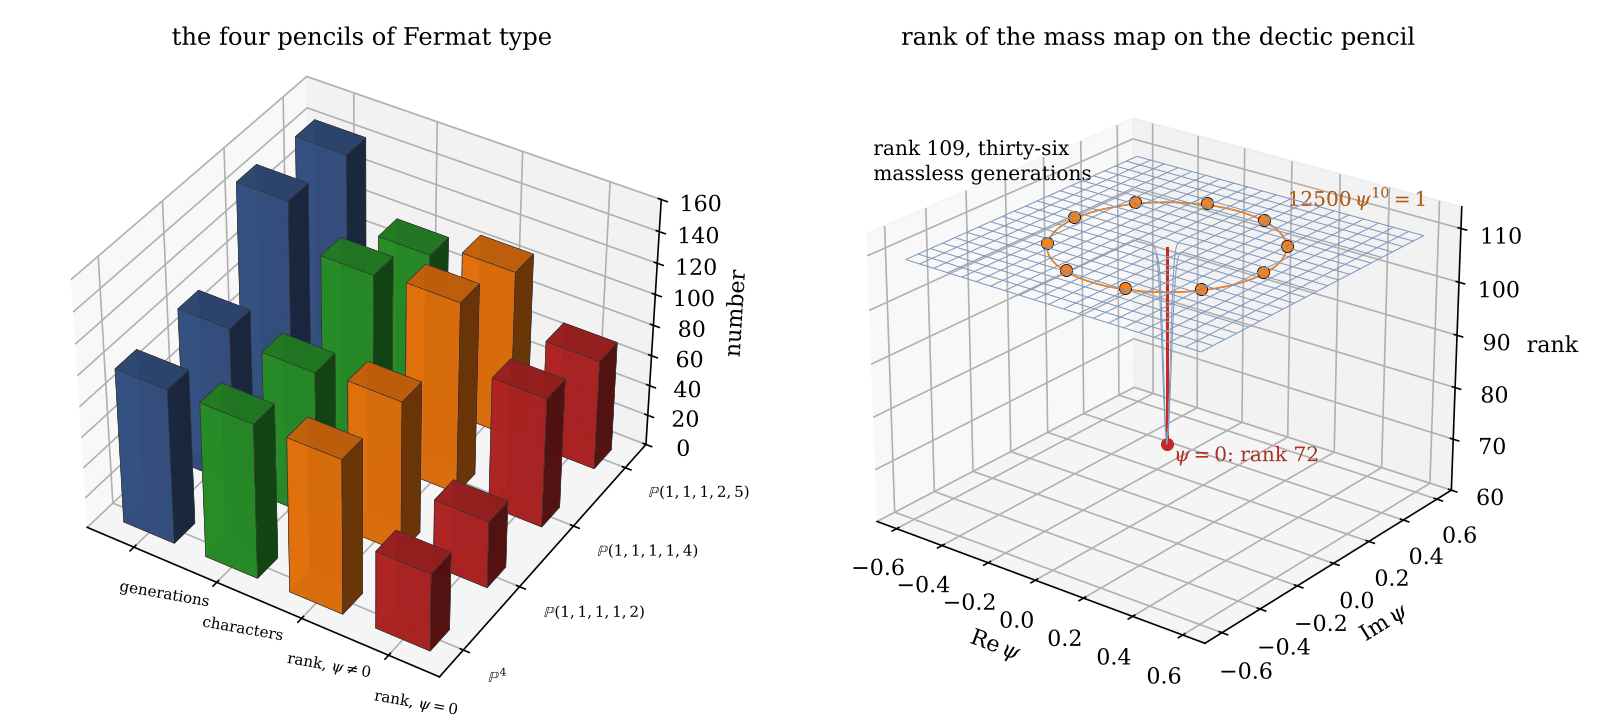
\includegraphics[width=0.96\textwidth]{figures/fig_weighted.png}
\caption{Left: for the quintic in $\PP^4$ and the sextic, octic and dectic
pencils in $\PP(1,1,1,1,2)$, $\PP(1,1,1,1,4)$ and $\PP(1,1,1,2,5)$, the
number of generations ($101$, $103$, $149$, $145$), the number of distinct
characters they carry ($101$, $96$, $122$, $100$), and the rank of the mass
map of the invariant direction for $\psi\ne0$ ($101$, $99$, $125$, $109$)
and at $\psi=0$ ($51$, $44$, $85$, $72$). Only on the quintic do the first
three bars agree. Right: the rank of the mass map over the $\psi$-plane of
the dectic pencil, $109$ off the Fermat point and $72$ at $\psi=0$ (the drop
is drawn with a small width); the ten points of the circle
$12\,500\,\psi^{10}=1$ are the singular members.}
\label{fig:weighted}
\end{figure}

\subsection{The socle functional}

Let $m_0=x^{\mathbf n-2\one}$, the monomial with exponents $n_i-2$; it has
degree $\sum_iw_i(n_i-2)=3d$. A monomial $x^{\ee}$ of degree $3d$ is in
sector $r\in\{0,\dots,d-1\}$ if $e_i\equiv n_i-2-r\pmod{n_i}$ for every
$i$. We then write
\begin{equation}\label{eq:wsector}
e_i=n_i-2-r+n_ik_i ;
\end{equation}
each $k_i$ is a nonnegative integer, since $k_i\le-1$ would give
$e_i\le-2-r$, and $\sum_ik_i=r$, by comparing degrees:
$\sum_iw_ie_i=5d-2d-rd+d\sum_ik_i=3d$.

\begin{theorem}[Weighted socle functional]\label{thm:wsocle}
Let $\psi^d\delta\ne1$. Then $m_0$ spans $R_{3d}$, and the functional
$\lambda$ on $R_{3d}$ with $\lambda(m_0)=1$ satisfies, for every monomial
$x^{\ee}$ of degree $3d$,
\[
\lambda(x^{\ee})=\begin{cases}\psi^r\prod_iw_i^{k_i}&\text{if $\ee$ is in
sector $r$, with $k$ as in \eqref{eq:wsector},}\\
0&\text{otherwise.}\end{cases}
\]
A monomial of degree $3d$ is in a sector if and only if its character is
trivial.
\end{theorem}

\begin{proof}
The character of $x^{\ee}$ is trivial when $\ee\equiv c\one$ modulo
$(n_1,\dots,n_5)$ for some integer $c$; taking $r\equiv-2-c\pmod d$ and
using $n_i\mid d$ this is the condition $e_i\equiv n_i-2-r$, so the
monomials with trivial character are those in a sector. Since $R_{3d}$ is
one-dimensional with trivial character, every monomial with a nontrivial
character vanishes in $R$.

Let $\ee$ be in sector $r\ge1$. We claim that some $i$ has $n_ik_i\ge
r+1$. Otherwise $k_i\le r/n_i=rw_i/d$ for every $i$, so $r=\sum_ik_i\le
r\sum_iw_i/d=r$, with equality only if $n_ik_i=r$ for every $i$; then every
$n_i$ divides $r$, and so does their least common multiple $d$, which is
impossible for $1\le r<d$. For such an $i$ we have $e_i\ge n_i-1$, and
\eqref{eq:wreduce} gives $x^{\ee}\equiv w_i\psi\,x^{\ee'}$ with
$e'_i=e_i-n_i+1$ and $e'_j=e_j+1$ for $j\ne i$; by \eqref{eq:wsector}
$\ee'$ is in sector $r-1$ with $k'_i=k_i-1$ and the other $k_j$ unchanged.
After $r$ steps we reach sector $0$, where all $k_i$ vanish and
$\ee=\mathbf n-2\one$. Collecting the factors,
$x^{\ee}\equiv\psi^r\prod_iw_i^{k_i}\,m_0$. Finally, $R_{3d}$ is spanned
by monomials, each of which is zero or a multiple of $m_0$, and
$R_{3d}\ne0$; so $m_0$ spans $R_{3d}$.
\end{proof}

\begin{corollary}\label{cor:wcouplings}
Let $\psi^d\delta\ne1$. The cubic form takes on three labels
$\va,\bb,\cc$ the value $\lambda(x^{\va+\bb+\cc})$, up to the normalisation
of $\lambda$: this is $\psi^r\prod_iw_i^{k_i}$ when $\va+\bb+\cc$ is in
sector $r$, and zero when the character of $x^{\va+\bb+\cc}$ is
nontrivial. In particular, for $\psi\ne0$ every coupling allowed by
$\Gamma$ is nonzero. This is Theorem~\ref{thm:E}(ii).
\end{corollary}

\subsection{The mass map}

The only label with trivial character is $h=\one$ for the sextic and
$h=(2,2,2,2,0)$ for the octic and the dectic: a label $\bb\equiv c\one$ has
$b_i=c$ for the coordinates of weight one, and the condition on the weight
leaves only these. So the invariant part of $R_d$ is spanned by $x^h$,
the invariant direction. For $\psi\ne0$ it contains the tangent vector
$\partial_\psi F_\psi=-dP$ of the pencil: for the sextic $P=x^h$, and for
the octic and the dectic $P=x^{\one}\equiv w_5\psi\,x^h$ by
\eqref{eq:wreduce} at $x_5$, whose exponent one equals $n_5-1$. By
Corollary~\ref{cor:wcouplings} the mass map of the invariant direction in
the basis of labels is
\[
M_{\bb\cc}=\lambda\big(x^{h+\bb+\cc}\big),\qquad \bb,\cc\in B .
\]
Since $h$ has trivial character, $M_{\bb\cc}\ne0$ requires
$[\cc]=-[\bb]$. For a character $\chi$ let $B_\chi$ be the set of labels
carrying it; then $M$ is the direct sum of the blocks on
$B_\chi\cup B_{-\chi}$, one for each pair $\{\chi,-\chi\}$ of characters
carried by labels (Proposition~\ref{prop:wchars} shows that $-\chi$ is
carried whenever $\chi$ is).

\begin{lemma}\label{lem:wminor}
Let $\psi\ne0$ and $\psi^d\delta\ne1$. Every entry of a block is
$\psi^r\prod_iw_i^{k_i}\ne0$. For $\bb,\bb'\in B_\chi$ and
$\cc,\cc'\in B_{-\chi}$ let $r$, $r'$, $\rho$, $\rho'$ be the sectors of
$h+\bb+\cc$, $h+\bb'+\cc'$, $h+\bb+\cc'$ and $h+\bb'+\cc$, and
$\Delta=r+r'-\rho-\rho'$. Then $\Delta\in\{-d,0,d\}$, and
\[
\begin{aligned}
&M_{\bb\cc}M_{\bb'\cc'}-M_{\bb\cc'}M_{\bb'\cc}\\
&\qquad=M_{\bb\cc'}M_{\bb'\cc}\big((\psi^d\delta)^{\Delta/d}-1\big),
\end{aligned}
\]
which vanishes exactly when $\Delta=0$.
\end{lemma}

\begin{proof}
The first statement is Theorem~\ref{thm:wsocle}, since each
$h+\bb+\cc$ in a block has trivial character. The two sums
$(h+\bb+\cc)+(h+\bb'+\cc')$ and $(h+\bb+\cc')+(h+\bb'+\cc)$ are equal, so
by \eqref{eq:wsector}, with $k,k',\kappa,\kappa'$ the vectors of the four
monomials, $n_i(k_i+k'_i-\kappa_i-\kappa'_i)=\Delta$ for every $i$. Hence
every $n_i$ divides $\Delta$, so $d$ does, and $|\Delta|<2d$ because the
sectors lie in $\{0,\dots,d-1\}$. The quotient of the two products is
$\psi^{\Delta}\prod_iw_i^{\Delta w_i/d}=(\psi^d\delta)^{\Delta/d}$.
\end{proof}

\begin{table}[t]
\caption{The blocks of the mass map of the invariant direction that
involve labels sharing a character. Each row gives the labels of
$B_\chi$ and of $B_{-\chi}$ in the notation of
Proposition~\ref{prop:wchars} (one representative of the orbit under
permutations of the coordinates of weight one), the number of such blocks,
the entries $M_{\bb\cc}$ with $\bb\in B_\chi$ in the order listed, and the
number of generations each block leaves massless for $\psi\ne0$; ``self''
means $-\chi=\chi$. All other blocks are a single label with $\chi=-\chi$
or a pair of single labels, and have full rank.}
\label{tab:wblocks}
\centering
\begin{tabular}{llllrr}
\toprule
pencil & $B_\chi$ & $B_{-\chi}$ & entries & blocks & massless\\
\midrule
sextic & $x_i^4x_5,\ x_j^2x_k^2x_l^2$ & $x_i^3x_jx_kx_l$ &
$2\psi^2;\ 1$ & $4$ & $1$\\
 & $x_i^3x_j^3,\ x_k^3x_l^3$ & self & $(2\psi^3,1;\ 1,2\psi^3)$ & $3$ & $0$\\
\midrule
octic & $x_i^6x_jx_k,\ x_j^3x_k^3x_l^2$ & $x_i^4x_jx_kx_l^2$ &
$4\psi^2;\ 1$ & $12$ & $1$\\
 & $x_i^6x_j^2,\ x_j^4x_k^2x_l^2$ & $x_j^6x_i^2,\ x_i^4x_k^2x_l^2$ &
$(16\psi^4,4\psi^2;\ 4\psi^2,1)$ & $6$ & $2$\\
 & $x_i^4x_j^4,\ x_k^4x_l^4$ & self & $(16\psi^4,1;\ 1,16\psi^4)$ & $3$ & $0$\\
\midrule
dectic & $x_i^2x_jx_kx_4^3,\ x_i^4x_j^3x_k^3$ & $x_i^2x_j^3x_k^3x_4$ &
$10\psi^2;\ 1$ & $3$ & $1$\\
 & $x_i^3x_jx_4^3,\ x_i^5x_j^3x_k^2$ & $x_ix_j^3x_k^4x_4$ &
$10\psi^2;\ 1$ & $6$ & $1$\\
 & $x_i^8x_jx_k,\ x_j^3x_k^3x_4^2$ & $x_i^4x_jx_kx_4^2$ &
$50\psi^4;\ 10\psi^2$ & $3$ & $1$\\
 & $x_i^7x_jx_4,\ x_ix_j^5x_k^4$ & $x_i^5x_jx_k^2x_4$ &
$50\psi^4;\ 1$ & $6$ & $1$\\
 & $x_i^8x_4,\ x_j^2x_k^2x_4^3,\ x_i^2x_j^4x_k^4$ & $x_i^4x_j^2x_k^2x_4$ &
$50\psi^4;\ 10\psi^2;\ 1$ & $3$ & $2$\\
 & $x_i^4x_4^3,\ x_i^6x_j^2x_k^2$ & $x_i^6x_4^2,\ x_j^4x_k^4x_4$ &
$(500\psi^6,10\psi^2;\ 50\psi^4,1)$ & $3$ & $2$\\
 & $x_i^8x_j^2,\ x_j^4x_k^2x_4^2$ & $x_j^8x_i^2,\ x_i^4x_k^2x_4^2$ &
$(250\psi^6,50\psi^4;\ 50\psi^4,10\psi^2)$ & $3$ & $2$\\
 & $x_i^6x_j^2x_4,\ x_j^6x_k^4$ & $x_i^6x_k^2x_4,\ x_k^6x_j^4$ &
$(50\psi^4,1;\ 1,250\psi^6)$ & $3$ & $0$\\
 & $x_i^6x_jx_kx_4,\ x_j^5x_k^5$ & self & $(50\psi^4,1;\ 1,250\psi^6)$ & $3$ & $0$\\
\bottomrule
\end{tabular}
\end{table}

\begin{proposition}\label{prop:wmass}
Let $\psi\ne0$ and $\psi^d\delta\ne1$. The blocks of the mass map that
involve labels sharing a character are those of Table~\ref{tab:wblocks}.
The mass map has rank $99$, $125$ and $109$ for the sextic, octic and
dectic, its kernel has dimension $4$, $24$ and $36$ and lies in the span of
the labels that share a character, and the rank is the same at every member
with $\psi\ne0$ and $\psi^d\delta\ne1$. At $\psi=0$ the mass map is the
matrix of the partial involution $\bb\mapsto\mathbf n-2\one-h-\bb$ on the
labels with $\bb\le\mathbf n-2\one-h$, of rank $44$, $85$ and $72$.
\end{proposition}

\begin{proof}
The classes of Proposition~\ref{prop:wchars} and their negatives give the
rows of Table~\ref{tab:wblocks}: for one representative of each orbit the
character $-\chi$ is computed from Lemma~\ref{lem:wwrap}, and the entries
from Theorem~\ref{thm:wsocle}; Appendix~\ref{app:wblocks} lists the sectors
and the vectors $k$. For example, for the sextic block with $i=1$,
$h+(3,1,1,1,0)+(4,0,0,0,1)=(8,2,2,2,2)$ is in sector $2$ with
$k=(1,0,0,0,1)$, which gives $2\psi^2$, and $h+(3,1,1,1,0)+(0,2,2,2,0)=
(4,4,4,4,1)=\mathbf n-2\one$ gives $1$. A block in which one of $B_\chi$,
$B_{-\chi}$ is a single label has the form $\left(\begin{smallmatrix}0&A\\
A^{\mathsf T}&0\end{smallmatrix}\right)$ with $A$ a row or a column of
nonzero entries, so it has rank two and leaves $|B_\chi|+|B_{-\chi}|-2$
generations massless, in the span of the class of two or three labels. For
a block with $2\times2$ matrix $A$, Lemma~\ref{lem:wminor} decides the
rank: $\Delta=0$ for the second octic row and the sixth and seventh dectic
rows, for instance $6+0-2-4=0$ in the sixth, so $A$ has rank one and two
generations on each side of the block are massless; $\Delta=\pm d$ for the
eighth dectic row and the three self-dual rows, whose determinants are
$4\psi^6-1$, $256\psi^8-1$ and $12\,500\psi^{10}-1$ up to nonzero
monomials, so these blocks have full rank. A single label with
$\chi=-\chi$, and a pair of single labels, give a block of full rank by the
first part of Lemma~\ref{lem:wminor}. Adding the last column of
Table~\ref{tab:wblocks}: $4\cdot1=4$, $12\cdot1+6\cdot2=24$ and
$3+6+3+6+3\cdot2+3\cdot2+3\cdot2=36$. None of the entries or
determinants depends on $\psi$ beyond these monomials and the factor
$\psi^d\delta-1$, so the rank is constant on the stated set.

At $\psi=0$ every sector $r\ge1$ gives zero, so $M_{\bb\cc}\ne0$ exactly
when $h+\bb+\cc=\mathbf n-2\one$. The vector
$\cc=\mathbf n-2\one-h-\bb$ has degree $3d-2d=d$ and entries at most
$n_i-2$, so it is a label exactly when $\bb\le\mathbf n-2\one-h$. Here
$\mathbf n-2\one-h=(3,3,3,3,0)$, $(4,4,4,4,0)$ and $(6,6,6,1,0)$, and the
labels below these vectors are counted by the coefficient of $t^6$ in
$(1+t+t^2+t^3)^4$, which is $44$, of $t^8$ in $(1+t+\dots+t^4)^4$, which is
$85$, and by $36+36=72$ solutions of $b_1+b_2+b_3+2b_4=10$ with $b_i\le6$
and $b_4\le1$.
\end{proof}

\subsection{Three families}

\begin{proposition}\label{prop:wthree}
Let $X$ be a member of the sextic, octic or dectic pencil with
$\psi^d\delta\ne1$, and $H$ a finite group acting freely on $X$. With the
standard embedding, $X/H$ does not have three net families.
\end{proposition}

\begin{proof}
By Theorem~\ref{thm:dictionary} the number of net families on $Y=X/H$ is
$|\chi(Y)|/2=|\chi(X)|/(2|H|)$, and three families need
$|H|=|\chi(X)|/6$, that is $34$ for the sextic and $48$ for the dectic; for
the octic $296/6$ is not an integer. Suppose $H$ has this order. The
projection $\pi\colon X\to Y$ is \'etale of degree $|H|$, $\chi(\cO_Y)=
\chi(\cO_X)/|H|=0$ and $c_1(Y)$ is torsion. As $H^2(X,\Q)=\Q L$ and $L$
generates $H^2(X,\Z)$ modulo torsion (Lemma~\ref{lem:wsmooth}), every line
bundle $D$ on $Y$ has $\pi^*D\equiv mL$ numerically for an integer $m$, and
these $m$ form a subgroup of $\Z$. It contains $|H|$: the line bundle
$\bigotimes_{g\in H}g^*\cO_X(1)$ is linearised by permuting its factors, so
it descends to $Y$, and it is numerically $|H|L$ because $H$ acts trivially
on $H^2(X,\Q)$. Let $m_0>0$ generate the subgroup and $D$ realise it. Then
$m_0$ divides $|H|$, and
\[
\begin{gathered}
D^3=\frac{m_0^3L^3}{|H|},\qquad c_2(Y)\cdot D=\frac{m_0\,c_2\cdot L}{|H|},\\
\chi(Y,D)=\frac{D^3}{6}+\frac{c_2(Y)\cdot D}{12},
\end{gathered}
\]
the last by Riemann--Roch with $c_1(Y)\equiv0$ and $\chi(\cO_Y)=0$. All
three numbers are integers. For the sextic, $D^3=3m_0^3/34$ forces
$34\mid m_0$, so $m_0=34$, $D^3=3468$, $c_2(Y)\cdot D=42$ and
$\chi(Y,D)=578+7/2$. For the dectic, $D^3=m_0^3/48$ forces $12\mid m_0$ and
$c_2(Y)\cdot D=17m_0/24$ forces $24\mid m_0$, so $m_0\in\{24,48\}$, with
$\chi(Y,D)=48+17/12$ and $384+17/6$. None is an integer, a contradiction.
\end{proof}

\begin{proof}[Proof of Theorem~\ref{thm:E}]
Smoothness and $h^{2,1}$ are Lemma~\ref{lem:wsmooth}, part (i) is
Proposition~\ref{prop:wchars}, part (ii) is
Corollary~\ref{cor:wcouplings}, part (iii) is Proposition~\ref{prop:wmass},
and part (iv) is Proposition~\ref{prop:wthree} together with
$|\chi(X)|/2\in\{102,148,144\}$ for $X$ itself.
\end{proof}

\begin{remark}[Why the quintic is different]\label{rem:wquintic}
On the quintic all $n_i$ equal five, so a shift moves every exponent by the
same amount and the wrapping count $\sum_ia_i=s$ of
Lemma~\ref{lem:wwrap} has no solution: this is the proof of
Theorem~\ref{thm:A}. When the $n_i$ differ, a wrap at a coordinate with
large $n_i$ can be balanced by wraps at the coordinate with $n_5=3$ or
$n_5=2$, and the shared classes of Proposition~\ref{prop:wchars} are
exactly these balances. The mass map then has blocks larger than $1\times1$
whose entries, all nonzero, satisfy $\Delta=0$, and these blocks carry the
massless generations. Among the four pencils, the quintic is therefore the
only one on which the characters of the symmetry group label the
generations and the invariant deformation gives every generation a mass.
\end{remark}

\section{The selection conjecture}\label{sec:selection}

\subsection{The landscape and its metric}

We use the setting of~\cite{Bha26a}. A heterotic vacuum is a pair $(X,V)$
of a Calabi--Yau threefold $X$ and a slope-polystable holomorphic bundle $V$
with $c_1(V)=0$ for which $c_2(T_X)-c_2(V)$ is effective; the standard
embedding is the case $V=T_X$. The landscape $\cL$ is the set of
isomorphism classes of vacua. It is the disjoint union of the components
$\cL_\tau$ of fixed topological type $\tau$, and each component carries the
Riemannian metric $g=G^{\WP}\oplus G^V$ made of the Weil--Petersson metric
of the complex structures and the $L^2$ metric of the bundle
moduli.\footnote{By the theorem of Bogomolov, Tian and Todorov the complex
structures of $X$ are unobstructed, and the bundle moduli of a stable
bundle are unobstructed when $H^2(X,\End_0V)=0$. Where a component is an
orbifold or has singular points, everything below is applied on its smooth
locus, or on orbifold charts; the only tools used are partitions of unity,
geodesic balls and cut-off functions, and all three exist in that
generality. As in~\cite{Bha26a} we take each $\cL_\tau$ to be a connected
manifold of finite dimension with countably many components in all.}
Mirror symmetry enters through an involution $\mu$ of a union $\cL^\mu$ of
components, which sends a vacuum to its mirror and is an isometry of $g$,
as~\cite{Bha26a} records for the Weil--Petersson metric. A vacuum is
\emph{viable} when it satisfies the nine conditions (C1)--(C9) of the
phenomenological closure theorem of~\cite{Bha26a}: anomaly cancellation and
stability, three net families, a Wilson line breaking to the Standard Model
group, three families without chiral exotics, masses for the vectorlike
exotics, doublet--triplet splitting, stabilised moduli, an acceptable rank
and hierarchy of the Yukawa masses, and consistent supersymmetry breaking.

\begin{conjecture}[Geometric Selection Conjecture~\cite{Bha26a}]
\label{conj:gsc}
There is a functional $\cS:\cL\to[0,\infty)$, constructed from the metric
$g$, such that
\begin{enumerate}[label=\textup{(G\arabic*)},leftmargin=*,itemsep=1pt]
\item $\cS$ is smooth and proper on each component $\cL_\tau$;
\item $\cS$ has a unique global minimum $\cV^\star\in\cL$;
\item $\cV^\star$ is viable;
\item $\cS\circ\mu=\cS$ on $\cL^\mu$.
\end{enumerate}
\end{conjecture}

\subsection{The functional adds nothing}

\begin{theorem}\label{thm:gscequiv}
Conjecture~\ref{conj:gsc} holds if and only if there is a viable vacuum
$\cV^\star$ with $\mu(\cV^\star)=\cV^\star$ whenever $\cV^\star\in\cL^\mu$.
\end{theorem}

\begin{proof}
Suppose $\cS$ exists, and let $\cV^\star$ be its minimum. It is viable by
(G3). If $\cV^\star\in\cL^\mu$, then $\cS(\mu\cV^\star)=\cS(\cV^\star)$ by
(G4), so $\mu\cV^\star$ is also a global minimum, and $\mu\cV^\star=
\cV^\star$ by (G2).

Conversely, let $\cV^\star$ be viable and fixed by $\mu$ when $\mu$ is
defined there, and let $\cL_{\tau^\star}$ be its component. The functional
is built in three steps.

\emph{A proper function on every component.} A second countable manifold
$M$ has a smooth proper function $\rho:M\to[0,\infty)$: take compact sets
$K_1\subset K_2\subset\cdots$ with $K_j$ inside the interior of $K_{j+1}$
and union $M$, a partition of unity $(\phi_j)$ with $\phi_j$ supported in
the interior of $K_{j+1}$ minus $K_{j-1}$, and $\rho=\sum_jj\phi_j$; then
$\rho\ge j$ outside $K_j$. Choose such a $\rho_\tau$ on every component. The
involution $\mu$ permutes the components of $\cL^\mu$, so on each orbit of
components we may replace $\rho$ by $\rho+\rho\circ\mu$, which is smooth,
proper (it is at least $\rho$) and $\mu$-invariant. Call the result $\rho$.

\emph{A quadratic well at $\cV^\star$.} Choose $r>0$ smaller than the
injectivity radius of $g$ at $\cV^\star$ and such that the closed geodesic
ball $\bar B$ of radius $r$ about $\cV^\star$ is compact. On the open ball
$B$ the function $f=d_g(\cV^\star,\cdot)^2$ is smooth, since it is the
squared norm of the inverse of the exponential map. If $\cV^\star\in
\cL^\mu$, then $\mu$ is an isometry fixing $\cV^\star$, so it preserves $B$
and $f\circ\mu=f$.

\emph{Gluing.} Let $\chi:[0,\infty)\to[0,1]$ be smooth, equal to $1$ on
$[0,r^2/4]$ and to $0$ on $[r^2/2,\infty)$, and extend $\chi\circ f$ by zero
outside $B$; the extension is smooth because $\chi\circ f$ vanishes on the
part of $B$ at distance more than $r/\sqrt2$ from $\cV^\star$. Put $c=r^2/4$
and
\[
\cS=(\chi\circ f)\,f+\big(1-\chi\circ f\big)\,(c+\rho)
\]
on $\cL_{\tau^\star}$, and $\cS=c+\rho$ on every other component. Then
$\cS$ is smooth and $\mu$-invariant, because every ingredient is. It
vanishes at $\cV^\star$ and nowhere else: where $\chi\circ f=1$ it equals
$f$, which vanishes only at $\cV^\star$; where $0<\chi\circ f<1$ it is a
convex combination of $f\ge r^2/4$ and $c+\rho\ge c$, both positive; and
where $\chi\circ f=0$ it equals $c+\rho\ge c$. So $\cV^\star$ is the unique
global minimum. Finally a sublevel set $\{\cS\le t\}$ of
$\cL_{\tau^\star}$ lies in $\bar B\cup\{\rho\le t-c\}$, a union of two
compact sets, and it is closed, so it is compact; on the other components
the sublevel sets of $c+\rho$ are compact. Thus $\cS$ satisfies (G1) to
(G4).
\end{proof}

Figure~\ref{fig:landscape} draws the functional of the proof on one
component.

\begin{figure}[t]
\centering
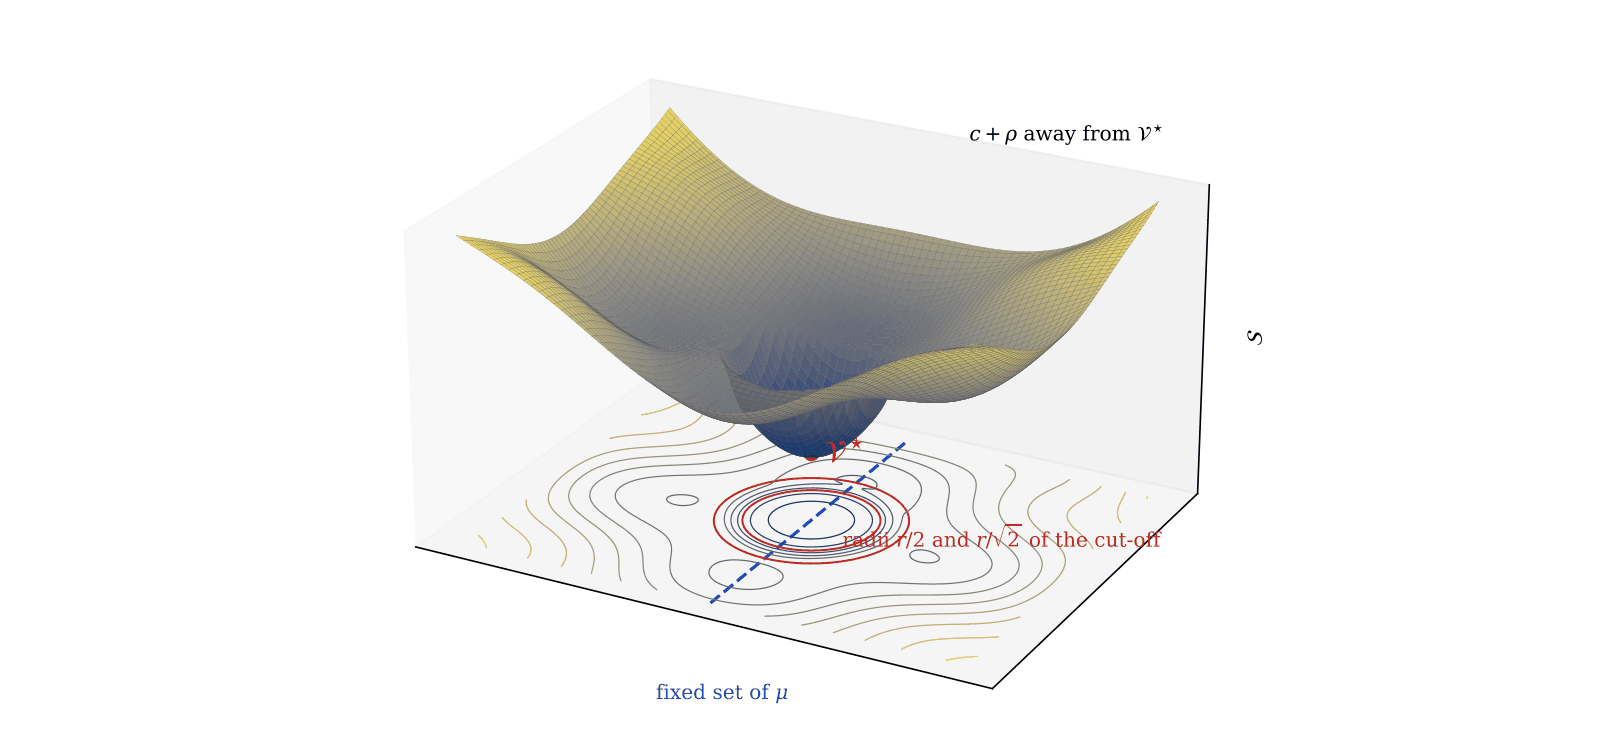
\includegraphics[width=0.9\textwidth]{figures/fig_landscape.png}
\caption{The functional $\cS$ of the proof of Theorem~\ref{thm:gscequiv}
on a two-dimensional component $\cL_{\tau^\star}$ on which $\mu$ acts by
a reflection (dashed line: its fixed set). Inside the radius $r/2$ about
$\cV^\star$ the functional is the squared distance $f$; outside the radius
$r/\sqrt2$ it is $c+\rho$ with $\rho$ proper and $\mu$-invariant; between
the two circles it is a convex combination of the two. The contour lines on
the floor are the level sets of $\cS$; all of them are compact, and the only
zero is $\cV^\star$.}
\label{fig:landscape}
\end{figure}

\begin{remark}[Constructed from the metric]\label{rem:frommetric}
The phrase ``constructed from the metric'' in Conjecture~\ref{conj:gsc} is
not a mathematical condition, and the strongest condition it can be read
as is invariance under a group of isometries of $(\cL,g)$. The proof gives
that reading as well: if $G$ is a compact group of isometries containing
$\mu$, averaging $\rho$ over $G$ with its Haar measure gives a $G$-invariant
smooth proper function (if $\int\rho(hx)\,dh\le t$ then $\rho(hx)\le t$ for
some $h$, so $x$ lies in the compact set $G\cdot\{\rho\le t\}$), and the
well at a $G$-fixed vacuum is $G$-invariant. So the conjecture in that
reading is equivalent to the existence of a viable vacuum fixed by $G$. In
every reading the functional is determined by the vacuum it selects and
contributes nothing else.
\end{remark}

\begin{remark}[Mirror pairs]
A viable vacuum outside the standard embedding lies outside $\cL^\mu$ when
$\mu$ is the mirror map of $(2,2)$ vacua, so the condition on $\mu$ in
Theorem~\ref{thm:gscequiv} is empty for it. If mirror pairs are identified
in $\cL$, as one point each, on the ground that they define the same
superconformal field theory, the condition is empty for every vacuum and
the conjecture is equivalent to the existence of one viable vacuum.
\end{remark}

\subsection{The Dwork pencil}

\begin{proposition}\label{prop:dworkselect}
\textup{(i)} For $\psi\ne0$ and $\psi^5\ne1$, the mass map of the invariant
direction $h$ on $X_\psi$ has rank $101$, its entries in the basis of
labels are $1$, $\psi$ and $\psi^2$, on $51$, $30$ and $20$ labels, and the
masses of Theorem~\ref{thm:C} are $|\psi|^{r(\bb)}$ times the Hodge factor
$(g_{\bb}g_{\sigma\bb})^{-1/2}$.

\textup{(ii)} Let $X$ be a smooth quintic threefold and $H$ a finite group
acting freely on $X$. The standard embedding on $X/H$ has
$100/|H|$ net families. In particular condition \textup{(C2)} fails on
$X/H$ for every such $H$, and no vacuum of the form $(X/H,T_{X/H})$ is
viable.

\textup{(iii)} On the sextic, octic and dectic pencils of
Section~\ref{sec:weighted}, with $\psi\ne0$ and $\psi^d\delta\ne1$, the
mass map of the invariant direction has a kernel of dimension $4$, $24$ and
$36$, and condition \textup{(C2)} fails on every member and on every
quotient of a member by a group acting freely.
\end{proposition}

\begin{proof}
Part (i) is Theorem~\ref{thm:C}. For (ii), a smooth quintic has
$h^{1,1}=1$ and $h^{2,1}=101$, so $\chi(X)=-200$. A free action multiplies
the Euler characteristic of the quotient by $1/|H|$, so
$\chi(X/H)=-200/|H|$, and by Theorem~\ref{thm:dictionary} the net number of
families is $|\chi(X/H)|/2=100/|H|$. Wilson lines on $X/H$ break the gauge
group but do not change this index. The equation $100/|H|=3$ has no
solution in integers, so (C2) fails. Part (iii) is
Propositions~\ref{prop:wmass} and~\ref{prop:wthree}.
\end{proof}

The proposition shows where the Dwork pencil stands with respect to the
conjecture. The condition on masses is met in the strongest form one can
ask of a single modulus: the mass matrix has full rank and three scales $1$,
$|\psi|$, $|\psi|^2$, which separate as $\psi\to0$. The pencil fails on the
count of families, and it fails there for every free quotient, so no
choice of Wilson lines rescues it. Three-family vacua satisfying (C1) to (C4)
exist on other threefolds: the heterotic standard models of Braun, He,
Ovrut and Pantev~\cite{BHOP05}, of Bouchard and Donagi~\cite{BD06}, and the
line-bundle models of Anderson, Gray, Lukas and Palti~\cite{AGLP11,AGLP12},
which also address (C5) and (C6). For none of them are (C7), (C8) and (C9)
established, and the words ``controlled'', ``acceptable'' and
``consistent'' in those conditions are fixed by comparison with
measurement, not by a definition. By Theorem~\ref{thm:gscequiv} this is the
whole of the open part of the Geometric Selection Conjecture. The weighted
pencils fail on both counts: they too never carry three families, and
their mass map leaves generations massless at every member.

\subsection{Free quotients of the one-parameter families}\label{sec:freequot}

The four pencils are four of the fourteen one-parameter families of
Calabi--Yau threefolds with $h^{1,1}=1$ whose Picard--Fuchs equations are
hypergeometric, listed by Doran and Morgan~\cite{DM06}. Thirteen of them are
complete intersections $X=X_{d_1,\dots,d_c}\subset\PP(w)$ of degrees
$d_1,\dots,d_c$ with $\sum_jd_j=\sum_iw_i$, whose general member is
quasi-smooth and misses the singular points of $\PP(w)$; they are the rows
of Table~\ref{tab:freequot}. The fourteenth, $X_{2,12}\subset
\PP(1,1,1,1,4,6)$, is not of this kind: its quadric involves only the four
coordinates of weight one, so it is not quasi-smooth at the point of
$\PP(4,6)$ where the equation of degree twelve vanishes, and we leave it
aside. For the thirteen, the count of families of
Proposition~\ref{prop:dworkselect} becomes a statement about every free
quotient, through one arithmetic invariant.

\begin{lemma}[Primes of a free action]\label{lem:freeprime}
Let $X$ be a compact K\"ahler threefold with $K_X\cong\cO_X$,
$h^{1,0}=h^{2,0}=0$, $b_2=1$ and $\pi_1(X)=0$, let $L$ be an ample line
bundle on $X$, and let $g$ be an automorphism of prime order $p$ without
fixed points. Then $p$ divides $\chi(X,kL)$ for every $k\ge1$.
\end{lemma}

\begin{proof}
Since $X$ is simply connected, $H^2(X,\Z)$ has no torsion, and since
$h^{0,1}=h^{0,2}=0$ the first Chern class identifies $\operatorname{Pic}X$
with $H^2(X,\Z)\cong\Z$. Let $A$ be its ample generator, so that $L=A^a$
with $a\ge1$. The bundle $g^*A$ is again an ample generator, so
$g^*A\cong A$. The obstruction to lifting the action of the cyclic group
$G=\langle g\rangle$ to $A$ lies in $H^2(G,\C^*)$, which vanishes for a
cyclic group, so $A$ and all its powers are $G$-linearised and $G$ acts on
$H^q(X,A^m)$. For $m\ge1$ these groups vanish in positive degree by
Kodaira's theorem, as $A^m=K_X\otimes A^m$ with $A^m$ ample. For $1\le
j<p$ the automorphism $g^j$ has no fixed points, and the holomorphic
Lefschetz formula of Atiyah and Bott~\cite{AB68} gives
$\sum_q(-1)^q\operatorname{tr}\big(g^j\,|\,H^q(X,A^m)\big)=0$, that is,
$\operatorname{tr}(g^j\,|\,H^0(X,A^m))=0$. A representation of $\Z/p$ whose
character vanishes off the identity is a multiple of the regular
representation, so $p$ divides $h^0(X,A^m)=\chi(X,A^m)$. Taking $m=ka$
gives the statement.
\end{proof}

\begin{table}[t]
\caption{The thirteen one-parameter complete intersections. The columns
give the type, the weights, the intersection numbers, the Euler
characteristic, the values $\chi(X,kL)=k^3L^3/6+k\,c_2\cdot L/12$ for
$k=1,2,3$, their greatest common divisor $g_X$, and the order $|\chi|/6$
that a free action giving three families would need.}
\label{tab:freequot}
\centering
\begin{tabular}{llrrrlrl}
\toprule
type & $w$ & $L^3$ & $c_2\cdot L$ & $\chi$ & $\chi(kL)$ & $g_X$ & $|\chi|/6$\\
\midrule
$X_5$ & $1^5$ & $5$ & $50$ & $-200$ & $5,15,35$ & $5$ & --\\
$X_6$ & $1^4,2$ & $3$ & $42$ & $-204$ & $4,11,24$ & $1$ & $34$\\
$X_8$ & $1^4,4$ & $2$ & $44$ & $-296$ & $4,10,20$ & $2$ & --\\
$X_{10}$ & $1^3,2,5$ & $1$ & $34$ & $-288$ & $3,7,13$ & $1$ & $48$\\
$X_{3,3}$ & $1^6$ & $9$ & $54$ & $-144$ & $6,21,54$ & $3$ & $24$\\
$X_{4,2}$ & $1^6$ & $8$ & $56$ & $-176$ & $6,20,50$ & $2$ & --\\
$X_{3,2,2}$ & $1^7$ & $12$ & $60$ & $-144$ & $7,26,69$ & $1$ & $24$\\
$X_{2,2,2,2}$ & $1^8$ & $16$ & $64$ & $-128$ & $8,32,88$ & $8$ & --\\
$X_{4,4}$ & $1^4,2^2$ & $4$ & $40$ & $-144$ & $4,12,28$ & $4$ & $24$\\
$X_{6,6}$ & $1^2,2^2,3^2$ & $1$ & $22$ & $-120$ & $2,5,10$ & $1$ & $20$\\
$X_{4,3}$ & $1^5,2$ & $6$ & $48$ & $-156$ & $5,16,39$ & $1$ & $26$\\
$X_{6,4}$ & $1^3,2^2,3$ & $2$ & $32$ & $-156$ & $3,8,17$ & $1$ & $26$\\
$X_{6,2}$ & $1^5,3$ & $4$ & $52$ & $-256$ & $5,14,31$ & $1$ & --\\
\bottomrule
\end{tabular}
\end{table}

\begin{proposition}\label{prop:freequot}
Let $X\subset\PP(w)$ be a quasi-smooth complete intersection of one of the
thirteen types of Table~\ref{tab:freequot} that misses the singular points
of $\PP(w)$, and let $H$ be a finite group acting freely on $X$. Then every
prime divisor of $|H|$ divides $g_X$. Hence $H$ is trivial for $X_6$,
$X_{10}$, $X_{3,2,2}$, $X_{6,6}$, $X_{4,3}$, $X_{6,4}$ and $X_{6,2}$; it is
a $5$-group for $X_5$, a $3$-group for $X_{3,3}$, and a $2$-group for
$X_8$, $X_{4,2}$, $X_{2,2,2,2}$ and $X_{4,4}$. With the standard embedding,
no free quotient of $X$ carries three net families.
\end{proposition}

\begin{proof}
As in Lemma~\ref{lem:wsmooth}, $X$ is a smooth threefold with $K_X\cong
\cO_X(\sum_jd_j-\sum_iw_i)=\cO_X$, and the Lefschetz theorem for
quasi-smooth complete intersections~\cite{Dol82} gives $h^{1,0}=h^{2,0}=0$
and $b_2=1$. For $\pi_1$, let $C\subset\C^{N}$ be the affine cone over $X$,
the zero set of the $c$ weighted homogeneous equations. Quasi-smoothness
says that $C$ is a complete intersection of dimension four with an isolated
singular point at the origin, so by Hamm's theorem~\cite{Ham71} its link
is $2$-connected; the weighted action of $\R_{>0}$ meets every sphere about
the origin once, so $C\setminus\{0\}$ is homotopy equivalent to the link and
is simply connected. As $X$ misses the points with nontrivial isotropy,
$\C^*$ acts freely on $C\setminus\{0\}$ with quotient $X$, and the exact
sequence of homotopy groups of this fibration gives $\pi_1(X)=0$.

Let $p$ be a prime divisor of $|H|$ and $g\in H$ an element of order $p$.
It has no fixed points, so by Lemma~\ref{lem:freeprime} with
$L=\cO_X(1)$, $p$ divides $\chi(X,kL)$ for all $k\ge1$. By Riemann--Roch,
with $c_1(X)=0$ and $\chi(\cO_X)=0$,
$\chi(X,kL)=k^3L^3/6+k\,c_2\cdot L/12$, a polynomial that takes integer
values and vanishes at $k=0$; writing it as $\alpha_1\binom k1+\alpha_2
\binom k2+\alpha_3\binom k3$ with integers $\alpha_i$, its values at all
$k\ge1$ have the same greatest common divisor as $\alpha_1,\alpha_2,
\alpha_3$, which is that of its values at $k=1,2,3$, the number $g_X$. The
intersection numbers are computed as in Lemma~\ref{lem:wsmooth}, from
$c(T_X)=\prod_i(1+w_iL)\prod_j(1+d_jL)^{-1}$ and
$L^3=\prod_jd_j/\prod_iw_i$, and give the table.

By Theorem~\ref{thm:dictionary} the quotient $X/H$ carries
$|\chi(X)|/(2|H|)$ net families, so three families need
$|H|=|\chi(X)|/6$. This is not an integer for $X_5$, $X_8$, $X_{4,2}$,
$X_{2,2,2,2}$ and $X_{6,2}$. In the remaining eight rows it is $34$, $48$,
$24$, $24$, $24$, $20$, $26$ or $26$, and each of these has a prime factor
not dividing $g_X$: $17$, $2$, $2$, $2$, $3$, $2$ and $2$ (twice).
\end{proof}

The proposition contains Theorem~\ref{thm:E}(iv) and
Proposition~\ref{prop:dworkselect}(ii) and strengthens them: the sextic and
dectic pencils admit no free action at all, and on a quintic every free
action is by a $5$-group, so that only the orders $5$ and $25$ divide
$|\chi|=200$ and a free quotient of a quintic has $20$ or $4$ families;
the quotient by $\Z/5\times\Z/5$ with four families is already
in~\cite{CHSW85}. For the five complete intersections in ordinary
projective space the free actions were classified by Braun~\cite{Bra11}
with a computer search; the proposition uses only the holomorphic
Lefschetz formula and Riemann--Roch.\footnote{On a quintic the group
$\Z/5\times\Z/5$ of~\cite{CHSW85}, generated by the cyclic permutation of
the coordinates and the diagonal phases $(1,\zeta,\zeta^2,\zeta^3,\zeta^4)$,
acts on the five coordinates through a central extension of order $125$,
the Heisenberg group, and $H^0(X,\cO_X(1))=\C^5$ is its irreducible
representation of dimension five; each cyclic subgroup of order five acts on
it by the regular representation, as Lemma~\ref{lem:freeprime} requires.}

\section{Conclusion}\label{sec:conclusion}

On the Dwork pencil the question of the title has a complete answer. The
hundred and one generations are labelled by characters of the symmetry
group $\Gamma$, each character occurring once; the couplings of three
generations are the values of one functional on the socle of the Jacobian
ring, equal to a power of the modulus when the symmetry allows them and to
zero otherwise; the invariant deformation pairs the generations by an
involution with a single fixed point, so its mass matrix is monomial with
determinant $\psi^{70}$; and at the Fermat point the masses are explicit
values of the Gamma function. The proofs use two facts only, the reduction
\eqref{eq:reduce} and the grading of the Jacobian ring by characters,
together with the general dictionary of Section~\ref{sec:dictionary}.

Two questions are not settled by the geometry of the pencil. The breaking
of $E_6$ to the Standard Model needs a free quotient and Wilson lines, and
on a quintic the number of families of a free quotient is $100/|H|$, never
three (Proposition~\ref{prop:dworkselect}), and the same holds for every
free quotient of the thirteen one-parameter complete intersections
(Proposition~\ref{prop:freequot}). The selection of the vacuum is
reduced by Theorem~\ref{thm:gscequiv} to the existence of one viable vacuum,
and that existence depends on conditions (C7) to (C9), whose thresholds are
set by measurement. The same two facts drive Section~\ref{sec:weighted},
where the three other one-parameter families of Fermat type are treated.
There the characters no longer separate the generations, the invariant
deformation leaves $4$, $24$ and $36$ of them massless at every member, and
no member or free quotient carries three families. Among the four pencils
of Fermat type, the quintic is the only one on which the symmetry labels
every generation and the invariant deformation gives every generation a
mass.

\section*{Data and code availability}

The programs that repeat the finite computations of this paper are in its
archive, release 1.2.0,
\url{https://github.com/creelie/strings/releases/tag/v1.2.0}~\cite{Repo},
which also holds the figures and the record of the engine runs. They are
written in C (the label and coupling counts), C++ (the expansion of the
Hessian by permutations), Python (all counts, the intersection numbers of
Appendix~\ref{app:fermat}, the Gamma values, and the labels, characters,
couplings and mass maps of the weighted pencils, and the intersection numbers,
values $\chi(X,kL)$ and invariants $g_X$ of Table~\ref{tab:freequot}), Julia (the Gamma values
and the intersection numbers), Macaulay2 (the Jacobian ring of the quintic
at two rational values of $\psi$, with the socle functional on all $3876$
monomials of degree fifteen and the Hessian, and the Jacobian rings of the
three weighted pencils at two rational values of $\psi$, with the socle
functional on every monomial of degree $3d$) and Lean~4 (the counts, the
arithmetic of the Hessian and the numbers of the weighted pencils, checked
by the kernel), with one shell script that runs all $215$ checks. No proof
in the paper depends on them. The constructions were organised on the
Anaxia engine~\cite{Ana26}, described in~\cite{BB26}; its
record for the five targets of this paper is part of the archive. The programs and the engine
runs were prepared by Deep Bhattacharjee with AI assistance from Claude
(Anthropic).

\section*{Ethical declarations}

\emph{Funding.} None. \emph{Competing interests.} None.

\appendix

\section{The Hessian in the socle}\label{app:hessian}

The Hessian matrix of $F_\psi$ has entries
\[
H_{ii}=20\,x_i^3,\qquad H_{ij}=-5\psi\prod_{k\ne i,j}x_k\quad(i\ne j).
\]
For a permutation $\pi$ of $\{1,\dots,5\}$ with $m$ moved points and
$f=5-m$ fixed points, the product $\prod_iH_{i\pi(i)}$ is
$20^f(-5\psi)^m$ times a monomial whose exponents are read off as follows.
A fixed coordinate $a$ receives $3$ from its diagonal entry and $1$ from each
of the $m$ off-diagonal entries, since an off-diagonal entry $(i,\pi(i))$
omits only the moved coordinates $i$ and $\pi(i)$. A moved coordinate $c$
is omitted by exactly two off-diagonal entries, those with $i=c$ and with
$\pi(i)=c$, which are different because $\pi(c)\ne c$; it receives $1$ from
each of the other $m-2$. Hence the monomial of $\pi$ is
\[
\prod_{a\ \mathrm{fixed}}x_a^{3+m}\prod_{c\ \mathrm{moved}}x_c^{m-2},
\]
of degree $f(3+m)+m(m-2)=15$, and it depends only on the number of moved
points. The five values of $m$ give:
\begin{itemize}[leftmargin=*,itemsep=1pt]
\item $m=0$: the monomial $m_0=(3,3,3,3,3)$, sector $0$;
\item $m=2$: $(5,5,5,0,0)$ up to order, sector $3$, so $\lambda=\psi^3$;
\item $m=3$: $(6,6,1,1,1)$ up to order, sector $2$, so $\lambda=\psi^2$;
\item $m=4$: $(7,2,2,2,2)$ up to order, sector $1$, so $\lambda=\psi$;
\item $m=5$: $(3,3,3,3,3)$, sector $0$.
\end{itemize}
The contribution of a permutation to $H(\psi)=\lambda(\Hess F_\psi)$ is
$\operatorname{sgn}(\pi)\,20^f(-5\psi)^m\psi^{r(m)}$ with $r(0)=r(5)=0$,
$r(2)=3$, $r(3)=2$, $r(4)=1$, so $m+r(m)=5$ for every $m\ge2$ and every
non-identity permutation contributes a multiple of $\psi^5$. The cycle
types are
\[
\begin{aligned}
&1^5:\ 1\ \text{permutation, }m=0,\ +20^5=3\,200\,000;\\
&2\,1^3:\ 10,\ \text{odd},\ m=2:\ 10\cdot(-1)\cdot20^3\cdot25=-2\,000\,000;\\
&3\,1^2:\ 20,\ \text{even},\ m=3:\ 20\cdot20^2\cdot(-125)=-1\,000\,000;\\
&4\,1:\ 30,\ \text{odd},\ m=4:\ 30\cdot(-1)\cdot20\cdot625=-375\,000;\\
&2^2\,1:\ 15,\ \text{even},\ m=4:\ 15\cdot20\cdot625=187\,500;\\
&5:\ 24,\ \text{even},\ m=5:\ 24\cdot(-3125)=-75\,000;\\
&3\,2:\ 20,\ \text{odd},\ m=5:\ 20\cdot(-1)\cdot(-3125)=62\,500,
\end{aligned}
\]
where the last six numbers are the coefficients of $\psi^5$. The counts
$1+10+20+30+15+24+20$ add up to $120$. The coefficients of $\psi^5$ add up
to $-3\,200\,000$, which gives $H(\psi)=3\,200\,000(1-\psi^5)$.

\section{The coupling count}\label{app:count}

\subsection{Ordered triples by sector}

For $\ee$ of degree fifteen, $O(\ee)$ is the number of ordered triples
$(\va,\bb,\cc)\in B^3$ with $\va+\bb+\cc=\ee$. We count it by the third
label: for each $\cc\in B$ with $\cc\le\ee$, put $\mathbf s=\ee-\cc$, a
vector of degree ten, and count the $\va\in B$ with $\mathbf s-\va\in B$,
that is, with
\[
\max(0,s_i-3)\le a_i\le\min(3,s_i)\quad\text{for all }i,\qquad
\textstyle\sum a_i=5.
\]
This number $N(\mathbf s)$ is the coefficient of $t^5$ in
$\prod_i\big(t^{\max(0,s_i-3)}+\dots+t^{\min(3,s_i)}\big)$. Write
$[n]=1+t+\dots+t^{n-1}$.

\emph{Sector $0$, $\ee=(3,3,3,3,3)$.} Here $\mathbf s=3\one-\cc$ has
entries in $\{0,\dots,3\}$, so $N(\mathbf s)$ is the coefficient of $t^5$ in
$\prod_i[s_i+1]$. The multiset of entries of $\mathbf s$ is the complement
of the type of $\cc$:
\[
\begin{array}{l|l|r|r}
\text{type of }\cc&\text{entries of }\mathbf s&\#\cc&N(\mathbf s)\\\hline
\{3,2,0,0,0\}&\{3,3,3,1,0\}&20&24\\
\{3,1,1,0,0\}&\{3,3,2,2,0\}&30&28\\
\{2,2,1,0,0\}&\{3,3,2,1,1\}&30&38\\
\{2,1,1,1,0\}&\{3,2,2,2,1\}&20&44\\
\{1,1,1,1,1\}&\{2,2,2,2,2\}&1&51
\end{array}
\]
The values of $N$ are central coefficients. For $\{3,3,3,1,0\}$,
$[4]^3=1+3t+6t^2+10t^3+12t^4+12t^5+\cdots$ and the factor $[2]$ gives
$12+12=24$. For $\{3,3,2,2,0\}$, $[4]^2=(1,2,3,4,3,2,1)$ and
$[3]^2=(1,2,3,2,1)$, so the coefficient is $2+6+12+6+2=28$. For
$\{3,3,2,1,1\}$, $[3][2]^2=(1,3,4,3,1)$ and the coefficient is
$2+9+16+9+2=38$. For $\{3,2,2,2,1\}$, $[3]^3=(1,3,6,7,6,3,1)$ and
$[4][2]=(1,2,2,2,1)$, so the coefficient is $3+12+14+12+3=44$. For
$\{2,2,2,2,2\}$ the coefficient of $t^5$ in $(1+t+t^2)^5$ is $51$. Hence
\[
O(3,3,3,3,3)=20\cdot24+30\cdot28+30\cdot38+20\cdot44+51=3391.
\]
(The table for $\ee=(3,3,3,3,3)$ also shows that every $\cc\in B$ occurs,
since $\mathbf s=3\one-\cc$ always admits some $\va$.)

\emph{Sector $1$, $\ee=(7,2,2,2,2)$.} Since $a_1+b_1\le6$, $c_1\ge1$, and
$c_i\le2$ for $i\ge2$. With $\mathbf s=\ee-\cc$, the entry $s_1=7-c_1$
forces $a_1\ge4-c_1$, and the remaining entries $s_i=2-c_i\le2$ impose only
$a_i\le s_i$. Grouping $\cc$ by $c_1$ and by the multiset of
$(c_2,\dots,c_5)$:
\[
\begin{array}{l|l|r|r|r}
c_1&(c_2,\dots,c_5)&\#\cc&N(\mathbf s)&\text{total}\\\hline
1&\{1,1,1,1\}&1&6&6\\
1&\{2,1,1,0\}&12&4&48\\
1&\{2,2,0,0\}&6&3&18\\
2&\{1,1,1,0\}&4&14&56\\
2&\{2,1,0,0\}&12&10&120\\
3&\{1,1,0,0\}&6&26&156\\
3&\{2,0,0,0\}&4&19&76
\end{array}
\]
For instance, when $c_1=3$ and $(c_2,\dots,c_5)=(2,0,0,0)$, $a_1$ ranges
over $\{1,2,3\}$ and the other entries satisfy $a_i\le(0,2,2,2)$ with sum
$5-a_1$; the coefficients of $t^4$, $t^3$, $t^2$ in $[3]^3$ are $6$, $7$,
$6$, which add to $19$. The total is $O(7,2,2,2,2)=480$.

\emph{Sector $2$, $\ee=(6,6,1,1,1)$.} Here $c_3,c_4,c_5\le1$, and the same
grouping gives
\[
\begin{array}{l|l|r|r|r}
\{c_1,c_2\}&(c_3,c_4,c_5)&\#\cc&N(\mathbf s)&\text{total}\\\hline
\{1,1\}&\{1,1,1\}&1&2&2\\
\{2,0\}&\{1,1,1\}&2&1&2\\
\{2,1\}&\{1,1,0\}&6&4&24\\
\{2,2\}&\{1,0,0\}&3&10&30\\
\{3,0\}&\{1,1,0\}&6&2&12\\
\{3,1\}&\{1,0,0\}&6&8&48\\
\{3,2\}&\{0,0,0\}&2&22&44
\end{array}
\]
and $O(6,6,1,1,1)=162$.

\emph{Sector $3$, $\ee=(5,5,5,0,0)$.} Here $c_4=c_5=0$ and
$c_1+c_2+c_3=5$. For $\{c_1,c_2,c_3\}=\{2,2,1\}$ the entries of
$\mathbf s$ are $(3,3,4)$, the bounds are $a_i\le3$ on the first two and
$1\le a_3\le3$, and the coefficient of $t^5$ in $[4]^2(t+t^2+t^3)$ is
$3+4+3=10$; for $\{3,1,1\}$ the entries are $(2,4,4)$ and the coefficient of
$t^5$ in $[3](t+t^2+t^3)^2$ is $2+3+2=7$; for $\{3,2,0\}$ the entries are
$(2,3,5)$ and the coefficient of $t^5$ in $[3][4](t^2+t^3)$ is $3+3=6$. With
three, three and six choices of $\cc$, $O(5,5,5,0,0)=30+21+36=87$.

The ordered counts by sector are $O_0=3391$, $O_1=5\cdot480=2400$,
$O_2=10\cdot162=1620$ and $O_3=10\cdot87=870$, with total $8281$ in
agreement with Section~\ref{sec:count}.

\subsection{Repeated labels}

For $\va\in B$ the partner $\cc$ with $2\va+\cc$ in a sector is found type
by type, as in the proof of Theorem~\ref{thm:C}. For $\va=\one$, $\cc=\one$
in sector $0$. For $\va$ of type $\{2,1,1,1,0\}$, sector $1$ gives
$c_i\equiv2-2a_i$, that is $\cc$ with a three where $\va$ has its two, a two
where $\va$ has its zero and zeros elsewhere, of sum five. For type
$\{3,1,1,0,0\}$, sector $1$ gives a one where $\va$ has its three, zeros
where it has ones and twos where it has zeros. For type $\{3,2,0,0,0\}$,
sector $2$ gives zero, two and ones. For type $\{2,2,1,0,0\}$, sector $3$
gives ones at the twos, a three at the one and zeros elsewhere. In each case
the other sectors produce a residue four or a total different from five.
So the hundred triples $\{\va,\va,\cc\}$ with $\cc\ne\va$ lie $20+30=50$ in
sector $1$, $20$ in sector $2$ and $30$ in sector $3$, and none in sector
$0$, which is the list $D_r=0,50,20,30$ used in Section~\ref{sec:count}.

\section{Hodge norms at the Fermat point}\label{app:fermat}

This appendix proves Proposition~\ref{prop:fermat}. Write
$G=\mu_5^5/\mu_5$ for the group of diagonal phases of $\PP^4$, which acts
on $X_0$. For $\mathbf k\in\{1,2,3,4\}^5$ with $\sum k_i\equiv0\pmod5$ let
$\chi_{\mathbf k}(a)=\zeta^{a\cdot\mathbf k}$.

\subsection{Eigenlines}

The character $\chi_{\mathbf k}$ occurs in $H^3(X_0,\C)$ exactly once, and
these are all the characters that occur: the number of such $\mathbf k$ is
$\frac15\sum_{j=0}^4\big(\sum_{k=1}^4\zeta^{jk}\big)^5=\frac15(4^5-4)=204
=b_3(X_0)$, and each occurs at least once because the residue
$\Res(x^{\mathbf k-\one}\Omega_0/F^{q+1})$, $5(q+1)=\sum k_i$, is a nonzero
class of character $\chi_{\mathbf k}$ (Griffiths' theorem and the fact that
$x^{\mathbf k-\one}$, with exponents at most three, is nonzero in the
Jacobian ring $\C[x]/(x_1^4,\dots,x_5^4)$ of the Fermat quintic). In
particular $\omega_{\bb}$ spans the line of $\mathbf k=\bb+\one$.

\subsection{The bilinear relation}

Let $Q$ be the intersection form on $H_3(X_0,\Z)$, extended to complex
coefficients, and identify $H^3$ with $H_3$ by Poincar\'e duality $D$, so
that $\int_c\omega=Q(c,D\omega)$ and $\int_{X_0}\omega\wedge\eta=
Q(D\omega,D\eta)$. Since $Q$ is $G$-invariant, it pairs the eigenline $L$ of
$\chi$ only with the eigenline $L'$ of $\bar\chi$. Let $e$ be an integral
cycle and $u$ its component in $L'$; its component in $L$ is $\bar u$,
because $e$ is real. If $D\omega_{\bb}=\alpha\bar u$ with $\bar u\ne0$, then
\[
\int_e\omega_{\bb}=Q(e,\alpha\bar u)=\alpha\,Q(u,\bar u),\qquad
\int_{X_0}\omega_{\bb}\wedge\overline{\omega_{\bb}}=|\alpha|^2Q(\bar u,u),
\]
and therefore
\begin{equation}\label{eq:bilinear}
g_{\bb}=\Big|\int_{X_0}\omega_{\bb}\wedge\overline{\omega_{\bb}}\Big|
=\frac{|\int_e\omega_{\bb}|^2}{|Q(u,\bar u)|}.
\end{equation}
It remains to compute both sides for one cycle.

\subsection{The cycle of Pham}

On the affine chart $x_5=1$ put $y_i=x_i/x_5$; the open part of $X_0$ is
$U=\{f=0\}$, $f=y_1^5+y_2^5+y_3^5+y_4^5+1$, and $\mu_5^4$ acts by
$y_i\mapsto\zeta^{a_i}y_i$. A character $\mathbf k$ of $G$ restricts to the
character $(k_1,k_2,k_3,k_4)$ of $\mu_5^4$, and $k_5\equiv-(k_1+k_2+k_3+
k_4)$. Pham~\cite{Pha65} showed that $U$ retracts onto the join of four
copies of the set of fifth roots of $-1$, and that $H_3(U,\Z)$ is generated
over $\Z[\mu_5^4]$ by the cycle
\[
e=(1-T_1)(1-T_2)(1-T_3)(1-T_4)\,\Delta,
\]
where $\Delta$ is the real simplex $\{y_i=\epsilon v_i,\ v_i\ge0,\
\sum v_i^5=1\}$ with $\epsilon^5=-1$, and $T_i$ multiplies $y_i$ by
$\zeta$.

\emph{The period.} By Griffiths' residue formula,
$\int_e\omega_{\bb}=\frac1{2\pi i}\int_{\tau(e)}x^{\bb}\Omega_0/F^2$ with
$\tau$ the tube map. On the chart this is the integral of
$y^{\bb'}dy/f^2$, $\bb'=(b_1,\dots,b_4)$. Put $f_s=\sum y_i^5+s$; then
$y^{\bb'}dy/f_s^2=-\partial_s(y^{\bb'}dy/f_s)$, and
$\frac1{2\pi i}\int_{\tau(e)}y^{\bb'}dy/f_s=\int_{e_s}y^{\bb'}dy/df_s$
with the Gelfand--Leray form. The substitution $y=s^{1/5}u$ shows that the
last integral is $s^{A}P$ with $A=\frac15\sum_{i\le4}k_i-1$ and $P$ its value
at $s=1$. Differentiating at $s=1$,
\[
\int_e\omega_{\bb}=-A\,P.
\]
On $\Delta$, with $t_i=v_i^5$, the Gelfand--Leray form is
$5^{-4}\prod_it_i^{1/5-1}dt$ on the simplex $\sum t_i=1$, and
$y^{\bb'}=\epsilon^{|\bb'|}\prod t_i^{b_i/5}$; Dirichlet's integral gives
$\int_\Delta=\epsilon^{|\bb'|+4}5^{-4}\prod_{i\le4}\Gamma(k_i/5)/
\Gamma(\sum_{i\le4}k_i/5)$, and each factor $1-T_i$ multiplies it by
$1-\zeta^{k_i}$. Since $\sum_{i\le4}k_i=10-k_5$, $A=1-k_5/5$ and
$\Gamma(A+1)=A\,\Gamma(A)$, so
\begin{equation}\label{eq:period}
\Big|\int_e\omega_{\bb}\Big|=5^{-4}\prod_{i=1}^4\big|1-\zeta^{k_i}\big|
\,\frac{\prod_{i=1}^4\Gamma(k_i/5)}{\Gamma(1-k_5/5)}.
\end{equation}

\emph{The intersection number.} For one variable, the reduced homology of
the fibre $\{y^5=-1\}$ is the augmentation ideal $I$ of $\Z[t]/(t^5-1)$,
the monodromy is multiplication by $t$, and the variation operator is
multiplication by $t-1$. The Seifert form $L(x,z)=\ip{x}{\mathrm{Var}^{-1}z}$
is therefore, in terms of the values $\hat x(k)=x(\zeta^k)$,
\[
L(x,z)=\frac15\sum_{k=1}^4\frac{\hat x(k)\,\hat z(-k)}{\zeta^{-k}-1}.
\]
By the theorem of Sebastiani and Thom~\cite{ST71}, in the form of
Sakamoto~\cite{Sak74} for Seifert forms, the Seifert form of
$y_1^5+\dots+y_4^5$ is, up to sign, the tensor product of four copies, and
the intersection form on the three-dimensional fibre is $Q=-L+L^{T}$. On the
eigenline of $(k_1,\dots,k_4)$ this gives
\[
Q(x,z)=\pm\frac1{5^4}\,\hat x(\mathbf k)\hat z(-\mathbf k)\Big(
\prod_{i\le4}\frac1{\zeta^{k_i}-1}-\prod_{i\le4}\frac1{\zeta^{-k_i}-1}\Big).
\]
With four factors, $\prod(\zeta^{k_i}-1)=\zeta^{\sum k_i}\prod(\zeta^{-k_i}
-1)$, so the bracket has absolute value
\[
\frac{|1-\zeta^{k_1+k_2+k_3+k_4}|}{\prod_{i\le4}|1-\zeta^{k_i}|^2}
=\frac{|1-\zeta^{k_5}|}{\prod_{i\le4}|1-\zeta^{k_i}|^2}.
\] The cycle $e$ has
$\hat e(\mathbf k)=\prod_{i\le4}(1-\zeta^{k_i})$ up to a unimodular factor,
so its component $u$ satisfies
\begin{equation}\label{eq:intersection}
|Q(u,\bar u)|=5^{-4}\prod_{i=1}^5\big|1-\zeta^{k_i}\big|.
\end{equation}
This is nonzero, so $\bar u\ne0$, as needed in \eqref{eq:bilinear}.

\subsection{Conclusion of the proof}

Inserting \eqref{eq:period} and \eqref{eq:intersection} in
\eqref{eq:bilinear},
\[
g_{\bb}=5^{-4}\,\prod_{i=1}^4\big|1-\zeta^{k_i}\big|\Gamma(k_i/5)^2\cdot
\frac{1}{|1-\zeta^{k_5}|\,\Gamma(1-k_5/5)^2}.
\]
With $|1-\zeta^k|=2\sin(\pi k/5)$ and $\Gamma(t)\Gamma(1-t)=\pi/\sin\pi t$,
\[
2\sin(\pi t)\,\Gamma(t)^2=2\pi\,\gamma(t),\qquad
\frac{1}{2\sin(\pi t)\,\Gamma(1-t)^2}=\frac{\gamma(t)}{2\pi},
\]
so $g_{\bb}=5^{-4}(2\pi)^3\prod_{i=1}^5\gamma(k_i/5)$, which is
\eqref{eq:gamma} with $C=(2\pi)^3/5^4$. The class of $\Omega$, with
$\mathbf k=\one$, has no derivative in the period computation, so
$|\int_e\Omega|=|P|$ with $\Gamma(\sum_{i\le4}k_i/5)=\Gamma(4/5)=
\Gamma(1-k_5/5)$, and the same formula holds: $\|\Omega\|^2=C\gamma(1/5)^5$.
Since $\partial_\psi\Res(\Omega_0/F_\psi)=\Res(5x_1\cdots x_5\Omega_0/
F_\psi^2)=5\omega_{\one}$ and $\omega_{\one}$ is of type $(2,1)$ at
$\psi=0$ (its character differs from that of $\Omega$), the
Weil--Petersson metric at the Fermat point is
\begin{align*}
G_{\psi\bar\psi}(0)&=\frac{25\,g_{\one}}{\|\Omega\|^2}
=25\,\frac{\gamma(2/5)^5}{\gamma(1/5)^5}\\
&=25\,\frac{\Gamma(2/5)^5\Gamma(4/5)^5}{\Gamma(1/5)^5\Gamma(3/5)^5}=0.19226.
\end{align*}

\subsection{Numerical values}

With $\Gamma(1/5)=4.59084$, $\Gamma(2/5)=2.21816$, $\Gamma(3/5)=1.48919$
and $\Gamma(4/5)=1.16423$, $\gamma(1/5)=3.94325$ and $\gamma(2/5)=1.48951$;
$\gamma(3/5)$ and $\gamma(4/5)$ are their inverses. The norms of the
five types follow by multiplying the five factors, and the masses of
Table~\ref{tab:fermat} are their inverses.

\section{Shared characters on the octic and the dectic}\label{app:wlabels}

\begin{table}[t]
\caption{The entries of the blocks of Table~\ref{tab:wblocks}, for the
representative with $(i,j,k,l)=(1,2,3,4)$. Exponent vectors are written in
full; the column $r$ is the sector of $h+\bb+\cc$ and $k$ is the vector of
\eqref{eq:wsector}.}
\label{tab:wblockdata}
\centering
\footnotesize
\begin{tabular}{lrlllrll}
\toprule
pencil & row & $\bb$ & $\cc$ & $h+\bb+\cc$ & $r$ & $k$ & entry\\
\midrule
sextic & 1 & $(4,0,0,0,1)$ & $(3,1,1,1,0)$ & $(8,2,2,2,2)$ & $2$ & $(1,0,0,0,1)$ & $2\psi^{2}$\\
 & 1 & $(0,2,2,2,0)$ & $(3,1,1,1,0)$ & $(4,4,4,4,1)$ & $0$ & $(0,0,0,0,0)$ & $1$\\
 & 2 & $(3,3,0,0,0)$ & $(3,3,0,0,0)$ & $(7,7,1,1,1)$ & $3$ & $(1,1,0,0,1)$ & $2\psi^{3}$\\
 & 2 & $(3,3,0,0,0)$ & $(0,0,3,3,0)$ & $(4,4,4,4,1)$ & $0$ & $(0,0,0,0,0)$ & $1$\\
 & 2 & $(0,0,3,3,0)$ & $(3,3,0,0,0)$ & $(4,4,4,4,1)$ & $0$ & $(0,0,0,0,0)$ & $1$\\
 & 2 & $(0,0,3,3,0)$ & $(0,0,3,3,0)$ & $(1,1,7,7,1)$ & $3$ & $(0,0,1,1,1)$ & $2\psi^{3}$\\
\midrule
octic & 1 & $(6,1,1,0,0)$ & $(4,1,1,2,0)$ & $(12,4,4,4,0)$ & $2$ & $(1,0,0,0,1)$ & $4\psi^{2}$\\
 & 1 & $(0,3,3,2,0)$ & $(4,1,1,2,0)$ & $(6,6,6,6,0)$ & $0$ & $(0,0,0,0,0)$ & $1$\\
 & 2 & $(6,2,0,0,0)$ & $(2,6,0,0,0)$ & $(10,10,2,2,0)$ & $4$ & $(1,1,0,0,2)$ & $16\psi^{4}$\\
 & 2 & $(6,2,0,0,0)$ & $(4,0,2,2,0)$ & $(12,4,4,4,0)$ & $2$ & $(1,0,0,0,1)$ & $4\psi^{2}$\\
 & 2 & $(0,4,2,2,0)$ & $(2,6,0,0,0)$ & $(4,12,4,4,0)$ & $2$ & $(0,1,0,0,1)$ & $4\psi^{2}$\\
 & 2 & $(0,4,2,2,0)$ & $(4,0,2,2,0)$ & $(6,6,6,6,0)$ & $0$ & $(0,0,0,0,0)$ & $1$\\
 & 3 & $(4,4,0,0,0)$ & $(4,4,0,0,0)$ & $(10,10,2,2,0)$ & $4$ & $(1,1,0,0,2)$ & $16\psi^{4}$\\
 & 3 & $(4,4,0,0,0)$ & $(0,0,4,4,0)$ & $(6,6,6,6,0)$ & $0$ & $(0,0,0,0,0)$ & $1$\\
 & 3 & $(0,0,4,4,0)$ & $(4,4,0,0,0)$ & $(6,6,6,6,0)$ & $0$ & $(0,0,0,0,0)$ & $1$\\
 & 3 & $(0,0,4,4,0)$ & $(0,0,4,4,0)$ & $(2,2,10,10,0)$ & $4$ & $(0,0,1,1,2)$ & $16\psi^{4}$\\
\midrule
dectic & 1 & $(2,1,1,3,0)$ & $(2,3,3,1,0)$ & $(6,6,6,6,0)$ & $2$ & $(0,0,0,1,1)$ & $10\psi^{2}$\\
 & 1 & $(4,3,3,0,0)$ & $(2,3,3,1,0)$ & $(8,8,8,3,0)$ & $0$ & $(0,0,0,0,0)$ & $1$\\
 & 2 & $(3,1,0,3,0)$ & $(1,3,4,1,0)$ & $(6,6,6,6,0)$ & $2$ & $(0,0,0,1,1)$ & $10\psi^{2}$\\
 & 2 & $(5,3,2,0,0)$ & $(1,3,4,1,0)$ & $(8,8,8,3,0)$ & $0$ & $(0,0,0,0,0)$ & $1$\\
 & 3 & $(8,1,1,0,0)$ & $(4,1,1,2,0)$ & $(14,4,4,4,0)$ & $4$ & $(1,0,0,1,2)$ & $50\psi^{4}$\\
 & 3 & $(0,3,3,2,0)$ & $(4,1,1,2,0)$ & $(6,6,6,6,0)$ & $2$ & $(0,0,0,1,1)$ & $10\psi^{2}$\\
 & 4 & $(7,1,0,1,0)$ & $(5,1,2,1,0)$ & $(14,4,4,4,0)$ & $4$ & $(1,0,0,1,2)$ & $50\psi^{4}$\\
 & 4 & $(1,5,4,0,0)$ & $(5,1,2,1,0)$ & $(8,8,8,3,0)$ & $0$ & $(0,0,0,0,0)$ & $1$\\
 & 5 & $(8,0,0,1,0)$ & $(4,2,2,1,0)$ & $(14,4,4,4,0)$ & $4$ & $(1,0,0,1,2)$ & $50\psi^{4}$\\
 & 5 & $(0,2,2,3,0)$ & $(4,2,2,1,0)$ & $(6,6,6,6,0)$ & $2$ & $(0,0,0,1,1)$ & $10\psi^{2}$\\
 & 5 & $(2,4,4,0,0)$ & $(4,2,2,1,0)$ & $(8,8,8,3,0)$ & $0$ & $(0,0,0,0,0)$ & $1$\\
 & 6 & $(4,0,0,3,0)$ & $(6,0,0,2,0)$ & $(12,2,2,7,0)$ & $6$ & $(1,0,0,2,3)$ & $500\psi^{6}$\\
 & 6 & $(4,0,0,3,0)$ & $(0,4,4,1,0)$ & $(6,6,6,6,0)$ & $2$ & $(0,0,0,1,1)$ & $10\psi^{2}$\\
 & 6 & $(6,2,2,0,0)$ & $(6,0,0,2,0)$ & $(14,4,4,4,0)$ & $4$ & $(1,0,0,1,2)$ & $50\psi^{4}$\\
 & 6 & $(6,2,2,0,0)$ & $(0,4,4,1,0)$ & $(8,8,8,3,0)$ & $0$ & $(0,0,0,0,0)$ & $1$\\
 & 7 & $(8,2,0,0,0)$ & $(2,8,0,0,0)$ & $(12,12,2,2,0)$ & $6$ & $(1,1,0,1,3)$ & $250\psi^{6}$\\
 & 7 & $(8,2,0,0,0)$ & $(4,0,2,2,0)$ & $(14,4,4,4,0)$ & $4$ & $(1,0,0,1,2)$ & $50\psi^{4}$\\
 & 7 & $(0,4,2,2,0)$ & $(2,8,0,0,0)$ & $(4,14,4,4,0)$ & $4$ & $(0,1,0,1,2)$ & $50\psi^{4}$\\
 & 7 & $(0,4,2,2,0)$ & $(4,0,2,2,0)$ & $(6,6,6,6,0)$ & $2$ & $(0,0,0,1,1)$ & $10\psi^{2}$\\
 & 8 & $(6,2,0,1,0)$ & $(6,0,2,1,0)$ & $(14,4,4,4,0)$ & $4$ & $(1,0,0,1,2)$ & $50\psi^{4}$\\
 & 8 & $(6,2,0,1,0)$ & $(0,4,6,0,0)$ & $(8,8,8,3,0)$ & $0$ & $(0,0,0,0,0)$ & $1$\\
 & 8 & $(0,6,4,0,0)$ & $(6,0,2,1,0)$ & $(8,8,8,3,0)$ & $0$ & $(0,0,0,0,0)$ & $1$\\
 & 8 & $(0,6,4,0,0)$ & $(0,4,6,0,0)$ & $(2,12,12,2,0)$ & $6$ & $(0,1,1,1,3)$ & $250\psi^{6}$\\
 & 9 & $(6,1,1,1,0)$ & $(6,1,1,1,0)$ & $(14,4,4,4,0)$ & $4$ & $(1,0,0,1,2)$ & $50\psi^{4}$\\
 & 9 & $(6,1,1,1,0)$ & $(0,5,5,0,0)$ & $(8,8,8,3,0)$ & $0$ & $(0,0,0,0,0)$ & $1$\\
 & 9 & $(0,5,5,0,0)$ & $(6,1,1,1,0)$ & $(8,8,8,3,0)$ & $0$ & $(0,0,0,0,0)$ & $1$\\
 & 9 & $(0,5,5,0,0)$ & $(0,5,5,0,0)$ & $(2,12,12,2,0)$ & $6$ & $(0,1,1,1,3)$ & $250\psi^{6}$\\
\bottomrule
\end{tabular}
\end{table}

This appendix completes the proof of Proposition~\ref{prop:wchars}. By
Lemma~\ref{lem:wwrap} it suffices to find, for each shift $s\le d/2$, the
labels $\bb$ with $b_i+s\not\equiv n_i-1\pmod{n_i}$ for every $i$ and
$\sum_ia_i=s$, and their images $\bb'$; the shift $d-s$ only reverses
these pairs, so two labels carry the same character exactly when they are
joined by a chain of the pairs found. For both pencils $n_5=2$ and
$b_5=0$, so the condition at $x_5$ excludes every odd shift, and for an
even shift $a_5=s/2$. In this appendix we drop the last coordinate, which
is zero, and write labels as vectors of length four.

\paragraph*{The octic.}
Here $b_i\le6$ and $b_1+b_2+b_3+b_4=8$, and the shifts to consider are
$s=2$ and $s=4$. Since $b_i+s\le10<16$, we have $a_i=1$ exactly when
$b_i\ge8-s$, and the excluded residue is $b_i=7-s$. So $\sum_ia_i=s$ asks
for exactly $s/2$ entries with $b_i\ge8-s$.

At $s=2$ exactly one entry equals six and none equals five, and the other
three entries add up to two. Up to a permutation of the coordinates this
leaves $(6,2,0,0)$ and $(6,1,1,0)$, with images $(0,4,2,2)$ and
$(0,3,3,2)$; there are twelve labels of each kind, which gives the $12+12$
pairs of Proposition~\ref{prop:wchars}(b). At $s=4$ exactly two entries are
at least four and none equals three; two entries of at least four already
add up to eight, so $\bb$ is a permutation of $(4,4,0,0)$, with image the
complementary permutation $(0,0,4,4)$, which gives three pairs.

The labels of the three lists are distinct: the sources at $s=2$ have an
entry six, their images have at most one entry larger than three, and the
labels at $s=4$ have two entries four and no entry six. So no label lies in
two pairs, the $27$ pairs are the classes, and the $149$ labels carry
$149-27=122$ characters.

\paragraph*{The dectic.}
Here $b_i\le8$ for $i\le3$, $b_4\le3$ and $b_1+b_2+b_3+2b_4=10$, and the
shifts to consider are $s=2$ and $s=4$. For $i\le3$, $b_i+s\le12<20$, so
$a_i=1$ exactly when $b_i\ge10-s$, and the excluded residue is
$b_i=9-s$. For $x_4$ we have $a_4=\lfloor(b_4+s)/5\rfloor$ and the excluded
residue is $b_4+s\equiv4\pmod5$. The condition is
\[
\#\{i\le3:\ b_i\ge10-s\}+a_4=s/2 .
\]

At $s=2$ the value $b_4=2$ is excluded, $a_4=1$ exactly when $b_4=3$, and
no $b_i$ equals seven. Either one $b_i$ equals eight and $b_4\le1$, which
leaves $(8,0,0,1)$, $(8,2,0,0)$ and $(8,1,1,0)$ up to a permutation of the
first three coordinates, with images $(0,2,2,3)$, $(0,4,2,2)$ and
$(0,3,3,2)$ under the same permutation; or no $b_i$ is at least eight and
$b_4=3$, which leaves the fifteen labels $(c_1,c_2,c_3,3)$ with
$c_1+c_2+c_3=4$, with images $(c_1+2,c_2+2,c_3+2,0)$.

At $s=4$ the value $b_4=0$ is excluded, so $b_4\ge1$ and $a_4=1$; hence
exactly one $b_i$ is at least six, and none equals five. The other entries
satisfy $b_j+b_k+2b_4=10-b_i\le4$ with $b_4\ge1$, which leaves
$(6,2,0,1)$, $(6,1,1,1)$, $(6,0,0,2)$, $(7,1,0,1)$ and $(8,0,0,1)$ up to
a permutation of the first three coordinates, with images $(0,6,4,0)$,
$(0,5,5,0)$, $(0,4,4,1)$, $(1,5,4,0)$ and $(2,4,4,0)$.

Sorting the labels of these lists by $b_4$ shows which of them coincide.
With $b_4=3$ there are the sources $(c_1,c_2,c_3,3)$ and the image
$(0,2,2,3)$, which is one of them, with $\cc=(0,2,2)$. With $b_4=2$ there
are $(0,4,2,2)$, $(0,3,3,2)$ and $(6,0,0,2)$, all different. With $b_4=1$
there are $(8,0,0,1)$, which occurs at both shifts, and $(6,2,0,1)$,
$(6,1,1,1)$, $(7,1,0,1)$ and $(0,4,4,1)$, all different. With $b_4=0$ there
are $(8,2,0,0)$ and $(8,1,1,0)$, the images $(c_1+2,c_2+2,c_3+2,0)$, all of
whose entries are at least two, and $(0,6,4,0)$, $(0,5,5,0)$, $(1,5,4,0)$
and $(2,4,4,0)$, of which only the last has all entries at least two; it is
the image of $\cc=(0,2,2)$. So the only chains longer than one pair are
\[
(8,0,0,1)\xrightarrow{s=2}(0,2,2,3)\xrightarrow{s=2}
(2,4,4,0)\xleftarrow{s=4}(8,0,0,1)
\]
and its permutations, the three triples of Proposition~\ref{prop:wchars}(c).
The remaining pairs are the $12$ with $\cc$ not a permutation of $(2,2,0)$
and the $6+3$ others at $s=2$, and the $6+3+3+6$ at $s=4$, which are the
pairs listed there: $39$ pairs and $3$ triples, $87$ labels in $42$ classes,
and $145-87+42=100$ characters.

\section{The blocks of the mass map}\label{app:wblocks}

Table~\ref{tab:wblockdata} gives the data behind Table~\ref{tab:wblocks}.
For each row we take the representative with $(i,j,k,l)=(1,2,3,4)$ and
list, for $\bb\in B_\chi$ and $\cc\in B_{-\chi}$ in the order of
Table~\ref{tab:wblocks}, the vector $h+\bb+\cc$, its sector $r$, the vector
$k$ of \eqref{eq:wsector} and the entry $\psi^r\prod_iw_i^{k_i}$ of
Theorem~\ref{thm:wsocle}. The other blocks of each row follow by permuting
the coordinates of weight one. For the blocks of size $2\times2$ the number
$\Delta$ of Lemma~\ref{lem:wminor} is $6$ for the self-dual sextic row, $0$
and $8$ for the second and third octic rows, and $0$, $0$, $10$ and $10$ for
the sixth to ninth dectic rows; for instance in the eighth dectic row
$\Delta=4+6-0-0=10$, so the determinant is
$50\cdot250\,\psi^{10}-1=12\,500\,\psi^{10}-1$.


\makeatletter\def\bibsection{\section*{References}}\makeatother
\begin{thebibliography}{99}\raggedright\advance\leftskip\labelwidth

\bibitem{CHSW85}
P.~Candelas, G.~T.~Horowitz, A.~Strominger and E.~Witten, Vacuum
configurations for superstrings, Nucl. Phys. B \textbf{258} (1985), 46--74,
\href{https://doi.org/10.1016/0550-3213(85)90602-9}{doi:10.1016/0550-3213(85)90602-9}.

\bibitem{Wit85}
E.~Witten, Symmetry breaking patterns in superstring models, Nucl. Phys. B
\textbf{258} (1985), 75--100,
\href{https://doi.org/10.1016/0550-3213(85)90603-0}{doi:10.1016/0550-3213(85)90603-0}.

\bibitem{Str85}
A.~Strominger, Yukawa couplings in superstring compactification, Phys. Rev.
Lett. \textbf{55} (1985), 2547--2550,
\href{https://doi.org/10.1103/PhysRevLett.55.2547}{doi:10.1103/PhysRevLett.55.2547}.

\bibitem{Can88}
P.~Candelas, Yukawa couplings between (2,1)-forms, Nucl. Phys. B
\textbf{298} (1988), 458--492,
\href{https://doi.org/10.1016/0550-3213(88)90351-3}{doi:10.1016/0550-3213(88)90351-3}.

\bibitem{CDGP91}
P.~Candelas, X.~C.~de la Ossa, P.~S.~Green and L.~Parkes, A pair of
Calabi--Yau manifolds as an exactly soluble superconformal theory, Nucl.
Phys. B \textbf{359} (1991), 21--74,
\href{https://doi.org/10.1016/0550-3213(91)90292-6}{doi:10.1016/0550-3213(91)90292-6}.

\bibitem{DGJ08}
C.~F.~Doran, B.~Greene and S.~Judes, Families of quintic Calabi--Yau 3-folds
with discrete symmetries, Commun. Math. Phys. \textbf{280} (2008), 675--725,
\href{https://doi.org/10.1007/s00220-008-0473-x}{doi:10.1007/s00220-008-0473-x}.

\bibitem{GP90}
B.~R.~Greene and M.~R.~Plesser, Duality in Calabi--Yau moduli space, Nucl.
Phys. B \textbf{338} (1990), 15--37,
\href{https://doi.org/10.1016/0550-3213(90)90622-K}{doi:10.1016/0550-3213(90)90622-K}.

\bibitem{DKL90}
L.~J.~Dixon, V.~Kaplunovsky and J.~Louis, On effective field theories
describing (2,2) vacua of the heterotic string, Nucl. Phys. B \textbf{329}
(1990), 27--82,
\href{https://doi.org/10.1016/0550-3213(90)90057-K}{doi:10.1016/0550-3213(90)90057-K}.

\bibitem{CdlO91}
P.~Candelas and X.~C.~de la Ossa, Moduli space of Calabi--Yau manifolds,
Nucl. Phys. B \textbf{355} (1991), 455--481,
\href{https://doi.org/10.1016/0550-3213(91)90122-E}{doi:10.1016/0550-3213(91)90122-E}.

\bibitem{Gri69}
P.~A.~Griffiths, On the periods of certain rational integrals, I, II, Ann.
of Math. \textbf{90} (1969), 460--541,
\href{https://doi.org/10.2307/1970746}{doi:10.2307/1970746}.

\bibitem{CG80}
J.~A.~Carlson and P.~A.~Griffiths, Infinitesimal variations of Hodge
structure and the global Torelli problem, in \emph{Journ\'ees de
g\'eom\'etrie alg\'ebrique d'Angers 1979}, Sijthoff and Noordhoff, Alphen
aan den Rijn, 1980, 51--76.

\bibitem{Hit74}
N.~Hitchin, Harmonic spinors, Adv. Math. \textbf{14} (1974), 1--55,
\href{https://doi.org/10.1016/0001-8708(74)90021-8}{doi:10.1016/0001-8708(74)90021-8}.

\bibitem{Han94}
A.~J.~Hanson, A construction for computer visualization of certain complex
curves, Notices Amer. Math. Soc. \textbf{41} (1994), 1156--1163.

\bibitem{BBCL16}
S.~Blesneag, E.~I.~Buchbinder, P.~Candelas and A.~Lukas, Holomorphic Yukawa
couplings in heterotic string theory, J. High Energy Phys. \textbf{2016},
no.~1, 152,
\href{https://doi.org/10.1007/JHEP01(2016)152}{doi:10.1007/JHEP01(2016)152}.

\bibitem{BMT24}
G.~Butbaia, D.~Mayorga Pe\~na, J.~Tan, P.~Berglund, T.~H\"ubsch, V.~Jejjala
and C.~Mishra, Physical Yukawa couplings in heterotic string
compactifications, Adv. Theor. Math. Phys. \textbf{28} (2024), 2783--2822,
\href{https://doi.org/10.4310/atmp.241119041341}{doi:10.4310/atmp.241119041341}.

\bibitem{DG88}
J.~Distler and B.~Greene, Some exact results on the superpotential from
Calabi--Yau compactifications, Nucl. Phys. B \textbf{309} (1988), 295--316,
\href{https://doi.org/10.1016/0550-3213(88)90084-3}{doi:10.1016/0550-3213(88)90084-3}.

\bibitem{Pha65}
F.~Pham, Formules de Picard--Lefschetz g\'en\'eralis\'ees et ramification
des int\'egrales, Bull. Soc. Math. France \textbf{93} (1965), 333--367,
\href{https://doi.org/10.24033/bsmf.1628}{doi:10.24033/bsmf.1628}.

\bibitem{ST71}
M.~Sebastiani and R.~Thom, Un r\'esultat sur la monodromie, Invent. Math.
\textbf{13} (1971), 90--96,
\href{https://doi.org/10.1007/BF01390095}{doi:10.1007/BF01390095}.

\bibitem{Sak74}
K.~Sakamoto, The Seifert matrices of Milnor fiberings defined by holomorphic
functions, J. Math. Soc. Japan \textbf{26} (1974), 714--721,
\href{https://doi.org/10.2969/jmsj/02640714}{doi:10.2969/jmsj/02640714}.

\bibitem{BHOP05}
V.~Braun, Y.-H.~He, B.~A.~Ovrut and T.~Pantev, A heterotic standard model,
Phys. Lett. B \textbf{618} (2005), 252--258,
\href{https://doi.org/10.1016/j.physletb.2005.05.007}{doi:10.1016/j.physletb.2005.05.007}.

\bibitem{BD06}
V.~Bouchard and R.~Donagi, An $SU(5)$ heterotic standard model, Phys. Lett.
B \textbf{633} (2006), 783--791,
\href{https://doi.org/10.1016/j.physletb.2005.12.042}{doi:10.1016/j.physletb.2005.12.042}.

\bibitem{AGLP11}
L.~B.~Anderson, J.~Gray, A.~Lukas and E.~Palti, Two hundred heterotic
standard models on smooth Calabi--Yau threefolds, Phys. Rev. D \textbf{84}
(2011), 106005,
\href{https://doi.org/10.1103/PhysRevD.84.106005}{doi:10.1103/PhysRevD.84.106005}.

\bibitem{AGLP12}
L.~B.~Anderson, J.~Gray, A.~Lukas and E.~Palti, Heterotic line bundle
standard models, J. High Energy Phys. \textbf{2012}, no.~6, 113,
\href{https://doi.org/10.1007/JHEP06(2012)113}{doi:10.1007/JHEP06(2012)113}.

\bibitem{Mor92}
D.~R.~Morrison, Picard--Fuchs equations and mirror maps for hypersurfaces,
in \emph{Essays on Mirror Manifolds}, International Press, Hong Kong, 1992,
241--264, \href{https://arxiv.org/abs/hep-th/9111025}{arXiv:hep-th/9111025}.

\bibitem{KT93}
A.~Klemm and S.~Theisen, Considerations of one-modulus Calabi--Yau
compactifications: Picard--Fuchs equations, K\"ahler potentials and mirror
maps, Nucl. Phys. B \textbf{389} (1993), 153--180,
\href{https://doi.org/10.1016/0550-3213(93)90289-2}{doi:10.1016/0550-3213(93)90289-2}.

\bibitem{Fon93}
A.~Font, Periods and duality symmetries in Calabi--Yau compactifications,
Nucl. Phys. B \textbf{391} (1993), 358--388,
\href{https://doi.org/10.1016/0550-3213(93)90152-F}{doi:10.1016/0550-3213(93)90152-F}.

\bibitem{Ste77}
J.~H.~M.~Steenbrink, Intersection form for quasi-homogeneous singularities,
Compositio Math. \textbf{34} (1977), 211--223.

\bibitem{Dol82}
I.~Dolgachev, Weighted projective varieties, in \emph{Group Actions and
Vector Fields}, Lecture Notes in Math. \textbf{956}, Springer, Berlin,
1982, 34--71,
\href{https://doi.org/10.1007/BFb0101508}{doi:10.1007/BFb0101508}.

\bibitem{AB68}
M.~F.~Atiyah and R.~Bott, A Lefschetz fixed point formula for elliptic
complexes. II. Applications, Ann. of Math. (2) \textbf{88} (1968),
451--491,
\href{https://doi.org/10.2307/1970721}{doi:10.2307/1970721}.

\bibitem{Ham71}
H.~A.~Hamm, Lokale topologische Eigenschaften komplexer R\"aume, Math. Ann.
\textbf{191} (1971), 235--252,
\href{https://doi.org/10.1007/BF01578709}{doi:10.1007/BF01578709}.

\bibitem{DM06}
C.~F.~Doran and J.~W.~Morgan, Mirror symmetry and integral variations of
Hodge structure underlying one-parameter families of Calabi--Yau
threefolds, in \emph{Mirror Symmetry V}, AMS/IP Stud. Adv. Math.
\textbf{38}, Amer. Math. Soc., Providence, RI, 2006, 517--537,
\href{https://doi.org/10.1090/amsip/038/22}{doi:10.1090/amsip/038/22}.

\bibitem{Bra11}
V.~Braun, On free quotients of complete intersection Calabi--Yau
manifolds, J. High Energy Phys. \textbf{2011} (2011), no.~4, 005,
\href{https://doi.org/10.1007/JHEP04(2011)005}{doi:10.1007/JHEP04(2011)005}.

\bibitem{Bha26a}
D.~Bhattacharjee, U.~Bhattacharya and S.~Ghosh, One missing axiom for the
complete closure of the heterotic landscape: resonance classifier of a
vibrating string creates the typical particle classes, Preprints.org (2026),
\href{https://doi.org/10.20944/preprints202603.0792.v2}{doi:10.20944/preprints202603.0792.v2}.

\bibitem{Bha26b}
D.~Bhattacharjee, P.~Samal, R.~Sadhu and S.~Singha Roy, Geometric
suppression of the electroweak scale from Calabi--Yau singularities,
Preprints.org (2026),
\href{https://doi.org/10.20944/preprints202603.0916.v1}{doi:10.20944/preprints202603.0916.v1}.

\bibitem{Bha25}
D.~Bhattacharjee, O.~Frederick, R.~Sadhu, S.~Bhattacharjee,
S.~Bhattacharya, S.~Nath Thakur, P.~Samal, P.~Nandi, T.~Bhattacharjee,
S.~Singha Roy, R.~Ghora and R.~Patra, Hopf-like fibrations on Calabi--Yau
manifolds, Preprints.org (2025),
\href{https://doi.org/10.20944/preprints202504.2581.v4}{doi:10.20944/preprints202504.2581.v4}.

\bibitem{Ana26}
D.~Bhattacharjee, BLLM: Beyond the LLM with Deep Human-Mind-AI, the Anaxia
engine, release 3.2.1, Zenodo (2026),
\href{https://doi.org/10.5281/zenodo.23524945}{doi:10.5281/zenodo.23524945};
all versions
\href{https://doi.org/10.5281/zenodo.23286641}{doi:10.5281/zenodo.23286641}.

\bibitem{BB26}
D.~Bhattacharjee and U.~Bhattacharya, BLLM: Beyond the LLM with Deep
Human-Mind-AI, paper distributed with the engine~\cite{Ana26} (2026).

\bibitem{Repo}
D.~Bhattacharjee, Which string vibrations become which generations on the
Dwork quintic: code, checks and engine record, release 1.2.0,
\url{https://github.com/creelie/strings/releases/tag/v1.2.0} (2026).

\end{thebibliography}

\end{document}
